%%% One-side print:
\documentclass[11pt,a4paper]{report}
\usepackage[top=25mm,bottom=25mm,right=25mm,left=30mm,head=12.5mm,foot=12.5mm]{geometry}
\usepackage{tikz}
\usetikzlibrary{calc,positioning,backgrounds,fit,arrows.meta}
\let\openright=\clearpage

%%% Two-side print:
%\documentclass[11pt,a4paper,twoside,openright]{report}
%\usepackage[top=25mm,bottom=25mm,right=25mm,left=30mm,head=12.5mm,foot=12.5mm]{geometry}
%\let\openright=\cleardoublepage

%%% DEFINITION OF BASIC VARIABLES
%\def\TypPrace{BP}                % bakalářská práce/bachelor thesis
\def\TypPrace{DP}               % diplomová práce/master thesis
%\def\Jazyk{cze}                  % čeština/czech
%\def\Jazyk{slo}                 % slovenština/slovak
\def\Jazyk{eng}                 % angličtina/english

%%% Definition of some useful macros
\input{makra}

%%% Název práce v jazyce práce (přesně podle zadání)
%%% Title of the thesis in the language used in the text (exact according to assignment)
\def\NazevPrace{A Data Integration Framework\\for Enterprise Application Security}

%%% Jméno autora
%%% Author's name - First name Surname
\def\AutorPrace{Bc. Vojtěch Kraus}

%%% Rok odevzdání a měsíc (slovně)
%%% Year of submission and month (verbally) - month YYYY
\def\DatumOdevzdani{May 2026}

%%% Vedoucí práce: Jméno a příjmení s~tituly
%%% Supervisor: First name and surname with titles
\def\Vedouci{Ing. Aleš Kotuč}

%%% Konzultant práce: Jméno a příjmení s~tituly
%%% Consultant: First name and surname with titles
\def\Konzultant{}

%%% Studijní program
%%% Study program
\def\StudijniProgram{Applied Data Analytics and Artificial Intelligence}

%%% Studijní program - specializace
%%% Study program - specialization
\def\Specializace{Retail and E-Commerce Data Analytics}

%%% Nepovinné poděkování (vedoucímu práce, konzultantovi, tomu, kdo zapůjčil software, literaturu apod.)
%%% Optional thanks (the supervisor, the consultant, the borrower of software, literature, etc.)
\def\Podekovani{%
I would like to thank Ing. Aleš Kotuč for his guidance and valuable feedback.
}

%%% Abstract (recommended range of about 150-250 words; this is not a thesis assignment)
%%% Only \AbstraktEN / \KlicovaSlovaEN are rendered; the Czech macros are kept
%%% for reference / possible reinstatement but are not included in the output.
\def\Abstrakt{%
Pro ochranu svých kriticky důležitých aplikací před kybernetickými hrozbami využívají podnikové bezpečnostní týmy řadu nástrojů k detekci a řešení zranitelností ve zdrojovém kódu aplikací, konfiguraci, závislostech, CI/CD pipeline a běhové infrastruktuře. Tyto nástroje používají různé integrační vzory, protokoly a datové formáty, což ztěžuje konzistentní parsování, deduplikaci, triáž a seskupování jejich nálezů. Ve velkých prostředích vznikají další výzvy při propojování všech nálezů s odpovídajícími podnikovými aplikacemi. Tato diplomová práce představuje datový rámec, který tyto výzvy řeší, a přináší tři odlišné přínosy: (1) specifikaci požadavků na datovou platformu pro bezpečnost aplikací, (2) znovupoužitelný a rozšiřitelný návrh pokrývající architekturu, datový model a datovou pipeline založenou na medallion architektuře, a (3) referenční implementaci postavenou na platformě Databricks. Tyto přínosy dohromady nabízejí bezpečnostním týmům základ pro vybudování robustní datové platformy nezávislé na jednotlivých dodavatelích kybernetické bezpečnosti, čímž je zbavují rizik obvykle spojených s vendor lock-inem.
}
\def\KlicovaSlova{aplikační bezpečnost, softwarová bezpečnost, DevSecOps, bezpečnostní integrace, konsolidace dat, medallion architektura, Databricks}

\def\AbstraktEN{%
To protect their business-critical applications from cybersecurity threats, enterprise security teams rely on numerous tools to detect and resolve vulnerabilities in application source code, configuration, dependencies, CI/CD pipelines, and runtime infrastructure. These tools use different integration patterns, protocols, and data formats, making it difficult to consistently parse, deduplicate, triage, and group their findings. In large environments, additional challenges emerge when linking all findings to the corresponding business applications. This thesis presents a data framework to tackle those challenges, delivering three distinct contributions: (1) a requirements specification for an application security data platform, (2) a reusable and extensible design covering architecture, data model, and medallion-based data pipeline, and (3) a reference implementation built on the Databricks platform. Together, these contributions offer application security teams a foundation for building a robust data platform independent of individual cybersecurity vendors, relieving them of risks usually associated with vendor lock-in.
}
\def\KlicovaSlovaEN{application security, software security, DevSecOps, security integration, data consolidation, medallion architecture, Databricks}

%%% Titulní strana a různé povinné informativní strany
%%% Title page and various mandatory information pages
\begin{document}
%%% Titulní strana práce a další povinné informační strany
%%% Title page of the thesis and other obligatory information pages

%%% Titulní strana práce
%%% Title page of the thesis

\pagestyle{empty}
\hypersetup{pageanchor=false}

%%% Use Latin Modern Sans for title page (not Fira Sans)
\begingroup
\fontfamily{lmss}\selectfont

\begin{center}
\Huge
\VSE\\
\FIS

\vspace{\stretch{1}}

\ifstringequal{\Jazyk}{eng}{
	
\includegraphics[width=.5\textwidth]{img/FIS_2_logo_2_rgb_EN}
}{
	\includegraphics[width=.5\textwidth]{img/FIS_2_logo_2_rgb_CZ}
}

\vspace{\stretch{2}}

\bfseries\NazevPrace

\vspace{8mm}
\mdseries\TypPraceText

\vspace{8mm}
\large
\begin{tabular}{rl}
\StudijniProgramText: & \StudijniProgram \\
\ifthenelse{\equal{\Specializace}{}}{%
	% empty value
	}{
	\rule{0pt}{6mm}%
	\SpecializaceText: & \Specializace \\
}
\end{tabular}

\vspace{\stretch{8}}

\begin{tabular}{rl}
\AutorText: & \AutorPrace \\
\noalign{\vspace{2mm}}
\VedouciText: & \Vedouci \\
\ifthenelse{\equal{\Konzultant}{}}{%
	% empty value
	}{
	\rule{0pt}{6mm}%
	\KonzultantText: & \Konzultant \\
}
\end{tabular}

\vspace{8mm}
\Praha, \DatumOdevzdani
\end{center}
\endgroup


%%% Prohlášení k použití AI / AI-use declaration
\hypersetup{pageanchor=true}
\cleardoublepage
\pagestyle{plain}
\openright
\vspace*{\fill}
\section*{\ProhlaseniAIText}
\noindent

I confirm that artificial intelligence tools were used in the preparation of
the submitted work. Specifically, they were used in the following ways:

\begin{itemize}
\item improvement of grammar, language style, and conciseness of the thesis, including review passes that shortened the manuscript by rephrasing longer prose and relocating detail into the attached product documentation,
\item generation of images and other media in the thesis,
\item generation of product documentation attached to the thesis (\texttt{docs.zip}),
\item generation of source code attached to the thesis (\texttt{mvp.zip}),
\item assistance with supporting tooling not submitted with the thesis, such as LaTeX build and continuous integration configuration and prose migration scripts.
\end{itemize}

{\leftskip=1.5em
Each use of any of the above methods is separately documented in an appendix to
the thesis, which provides a more detailed explanation of which tool was used in
which specific part of the work; the author's own contribution is highlighted.

I confirm that:
\begin{itemize}
\item my work is original and was prepared in accordance with ethical standards, in particular the Code of Ethics of the Prague University of Economics and Business; that all information sources used are properly cited in the work; and that any generated content has been verified by me;
\item I accept full responsibility for the entire content of the thesis.
\end{itemize}
}

\vspace{1cm}



%%% Poděkování
%%% Acknowledgments
\hypersetup{pageanchor=true}
\cleardoublepage
\pagestyle{plain}
\openright
\vspace*{\fill}
\section*{\PodekovaniText}
\noindent
\Podekovani
\vspace{1cm}


%%% Povinná informační strana práce
%%% Obligatory information page of the thesis
\openright
\section*{Abstract}
\noindent
\AbstraktEN
\subsection*{Keywords}
\noindent
\KlicovaSlovaEN

\openright


%%% Strana s automaticky generovaným obsahem práce
%%% A page with automatically generated content of the thesis
\setcounter{tocdepth}{2}
\tableofcontents

%%% Seznam obrázků v práci
%%% List of figures in the thesis
\openright
\listoffigures

%%% Seznam tabulek v práci (volitelně)
%%% List of tables in the thesis (optionally)
\clearpage
\listoftables

%%% Seznam zdrojových kódů v práci (volitelně)
%%% List of source listings in the thesis (optionally)
\clearpage
\lstlistoflistings

%%% Seznam zkratek v práci (volitelně)
%%% List of abbreviations in the thesis (optionally)
\printglossary[type=\acronymtype,title={\SeznamZkratek}]

\pagestyle{fancyx}
%%% Jednotlivé kapitoly práce jsou pro přehlednost uloženy v samostatných souborech
%%% The individual chapters of the thesis are stored in separate files for clarity
{%
\pagestyle{plain}
% \chapter*{Recommendations for the preparation of thesis at FIS}

\begin{quote}
\bfseries\itshape
This part of the template does not normally belong to the thesis. For the final
text is needed:
\begin{itemize}
\item in file \verb|thesis.tex| delete line \verb|\chapter*{Recommendations for the preparation of thesis at FIS}

\begin{quote}
\bfseries\itshape
This part of the template does not normally belong to the thesis. For the final
text is needed:
\begin{itemize}
\item in file \verb|thesis.tex| delete line \verb|\chapter*{Recommendations for the preparation of thesis at FIS}

\begin{quote}
\bfseries\itshape
This part of the template does not normally belong to the thesis. For the final
text is needed:
\begin{itemize}
\item in file \verb|thesis.tex| delete line \verb|\include{recommendation}|
\item and possibly also an unnecessary file \verb|recommendation.tex|
\end{itemize}
\end{quote}

The following thesis recommendations (hereinafter referred to as 
"recommendations") are intended to evaluate the defensibility of the thesis. 
They are intended for all types of theses in all Bachelor's and Master's degree 
programmes. They are not a substitute for thesis evaluations. If the committee 
considers the thesis undefensible, it should argue that an item in these 
recommendations has not been met.

\section*{Work done}
\begin{itemize}
\item \vspace*{-2ex}The student has carried out professional work in the field of his/her study programme (including interdisciplinary areas).
\item The final thesis demonstrates the student's orientation in the chosen field and his/her ability to define and achieve the chosen goal in this field. 
\item The student has done professional work of a workload in the range of months.
\end{itemize}

\section*{Objectives and context}
\begin{itemize}
\item \vspace*{-2ex}The text of the thesis describes the background - the expert context on which the student is based - the situation in professional knowledge or the situation in a specific application case.
\item The starting points contain only the findings that have an impact on the results of the thesis.
\item The text of the thesis clearly describes the aim of the thesis; if the aim is to solve a problem, the problem is sufficiently defined.
\item The reasonableness of the objectives in relation to the baseline is argued.
\item The specificity of the main objective is argued in the text - it is not a generic problem, which has been solved in the same way many times.
\item The formulation of the aim refers to a professional problem, not to the text of the thesis itself, to the reader or to the author. Thus, the objective is not formulated as "to write a text", "to communicate to the reader", "to describe the issue", "to explain", "to become familiar with the literature in the field", etc.
\item The text of the thesis is professional, not popular science. It solves a professional (practical or theoretical) problem.
\end{itemize}

\section*{Methodology}
\begin{itemize}
\item \vspace*{-2ex}The text of the final thesis describes the process by which the student worked, separately from the results.
\item The procedure is described in steps, from which you can estimate their laboriousness.
\item The procedure lists all the work the student has done. If there are steps in the procedure that the student has not done, they are clearly marked as such (and the reason is given).
\item The procedure is described in such a way that if someone else followed it, they would get similar results as the student.
\item The procedure is described in concrete terms, not just using generic names of thought processes such as analysis, deduction, synthesis, etc.
\item If the procedure used follows established methods described in the literature, it is not necessary to explain their operation in detail. However, the student should justify his/her choice of methods used or describe the deviations of the actual procedure from the established methods.
\end{itemize}

\section*{Results}
\begin{itemize}
\item \vspace*{-2ex}The results demonstrate that the student has carried out expert work in the field of the study programme (including interdisciplinary areas).
\item From the wording of the text of the final thesis it is clear what is the original result of the student, what is a fact taken from sources and what is speculation or discussion of results.
\item The text describes and interprets the results according to the procedure.
\item The text describes the partial results as outputs of the individual steps. Less important results are presented in the appendices, so that the text remains clear.
\item It is documented that the individual steps (e.g. calculations, descriptive statistics, interview records, program code, researcher's diary, etc.) have been performed, e.g. by uploading attachments to InSIS.
\item The text of the thesis describes the scientific results in a logical flow of argumentation. 
\end{itemize}

\section*{Conclusions}
\begin{itemize}
\item \vspace*{-2ex}Conclusions assess the degree to which the objective has been met.
\item The conclusions argue how the results have contributed to solving the problem.
\item Conclusions describe the possible impact of the results on the context (situation in the professional environment or in a specific application case), e.g. possible further work.
\item The conclusions mention possible limitations of the results obtained.
\end{itemize}

\section*{Originality}
\begin{itemize}
\item \vspace*{-2ex}All adopted, translated or paraphrased texts are properly marked and cited in accordance with citation standard APA 7 (we recommend using the Zotero citation tool).
\item In the case of the use of automatic text generation tools, this is in accordance with the rules and methodological recommendations of the Prague University of Economics and Business.
\item The text of the thesis cites and paraphrases only the sources that were used to solve the problem or define the context.
\item The text of the thesis does not unnecessarily recapitulate obvious theoretical knowledge (e.g. from the basic courses of the study programme).
\item In exceptional cases, if the student did not work completely alone, the collaborators (company, academic) and the student's contribution to their performance are indicated at each step of the procedure or in the form of a table in an appendix.
\end{itemize}

\section*{Form}
\begin{itemize}
\item \vspace*{-2ex}The text of the thesis is written as a coherent structured text, as paragraphs divided into chapters, in a structure suitable for the problem addressed.
\item Pages, tables, figures, appendices (etc.) are numbered.
\item Tables, figures, appendices, program code (etc.) that are not referenced from the body of the text do not appear in the thesis.
\item The format of the thesis is in accordance with the recommendations available on the FIS intranet for students.
\item The final thesis may take the form of a scientific article. In this case, it may be accompanied by an explanatory introduction (e.g. description of the journal, review process, co-authorship of the thesis supervisor, etc.).
\end{itemize}

\section*{Additional requirements for the thesis}
\begin{itemize}
\item \vspace*{-2ex}The diploma thesis significantly deepens the field of knowledge in the given topic.
\item The thesis clearly specifies the author's own contribution, which is in line with the objectives of the thesis. 
\item It is necessary to validate the results of the thesis (e.g. comparison of the results obtained with the literature, mathematical proof, structured interviews with interest groups, exact testing/measurement of results, etc.).
\end{itemize}

\section*{Specifics of team theses}
\begin{itemize}
\item \vspace*{-2ex}The fact that the thesis will be carried out in a team must be stated in the Thesis Assignment stored in InSIS and therefore approved by the thesis supervisor and the guarantor of the study programme (specialisation).
\item Each student in the team submits an individual thesis, which is individually assessed, individually defended and evaluated. Each student is responsible for the entire text of the thesis.
\item Only a small part of the thesis may be shared in cases approved by the thesis advisor. More than 70% of the thesis is individual.
\item The artifacts produced by the team should be published in Git or on the project wiki, for example, and referenced by the authors of the thesis.
\item Each thesis completed by the team includes an appendix entitled Team Members' Contribution to the Result.
\end{itemize}
|
\item and possibly also an unnecessary file \verb|recommendation.tex|
\end{itemize}
\end{quote}

The following thesis recommendations (hereinafter referred to as 
"recommendations") are intended to evaluate the defensibility of the thesis. 
They are intended for all types of theses in all Bachelor's and Master's degree 
programmes. They are not a substitute for thesis evaluations. If the committee 
considers the thesis undefensible, it should argue that an item in these 
recommendations has not been met.

\section*{Work done}
\begin{itemize}
\item \vspace*{-2ex}The student has carried out professional work in the field of his/her study programme (including interdisciplinary areas).
\item The final thesis demonstrates the student's orientation in the chosen field and his/her ability to define and achieve the chosen goal in this field. 
\item The student has done professional work of a workload in the range of months.
\end{itemize}

\section*{Objectives and context}
\begin{itemize}
\item \vspace*{-2ex}The text of the thesis describes the background - the expert context on which the student is based - the situation in professional knowledge or the situation in a specific application case.
\item The starting points contain only the findings that have an impact on the results of the thesis.
\item The text of the thesis clearly describes the aim of the thesis; if the aim is to solve a problem, the problem is sufficiently defined.
\item The reasonableness of the objectives in relation to the baseline is argued.
\item The specificity of the main objective is argued in the text - it is not a generic problem, which has been solved in the same way many times.
\item The formulation of the aim refers to a professional problem, not to the text of the thesis itself, to the reader or to the author. Thus, the objective is not formulated as "to write a text", "to communicate to the reader", "to describe the issue", "to explain", "to become familiar with the literature in the field", etc.
\item The text of the thesis is professional, not popular science. It solves a professional (practical or theoretical) problem.
\end{itemize}

\section*{Methodology}
\begin{itemize}
\item \vspace*{-2ex}The text of the final thesis describes the process by which the student worked, separately from the results.
\item The procedure is described in steps, from which you can estimate their laboriousness.
\item The procedure lists all the work the student has done. If there are steps in the procedure that the student has not done, they are clearly marked as such (and the reason is given).
\item The procedure is described in such a way that if someone else followed it, they would get similar results as the student.
\item The procedure is described in concrete terms, not just using generic names of thought processes such as analysis, deduction, synthesis, etc.
\item If the procedure used follows established methods described in the literature, it is not necessary to explain their operation in detail. However, the student should justify his/her choice of methods used or describe the deviations of the actual procedure from the established methods.
\end{itemize}

\section*{Results}
\begin{itemize}
\item \vspace*{-2ex}The results demonstrate that the student has carried out expert work in the field of the study programme (including interdisciplinary areas).
\item From the wording of the text of the final thesis it is clear what is the original result of the student, what is a fact taken from sources and what is speculation or discussion of results.
\item The text describes and interprets the results according to the procedure.
\item The text describes the partial results as outputs of the individual steps. Less important results are presented in the appendices, so that the text remains clear.
\item It is documented that the individual steps (e.g. calculations, descriptive statistics, interview records, program code, researcher's diary, etc.) have been performed, e.g. by uploading attachments to InSIS.
\item The text of the thesis describes the scientific results in a logical flow of argumentation. 
\end{itemize}

\section*{Conclusions}
\begin{itemize}
\item \vspace*{-2ex}Conclusions assess the degree to which the objective has been met.
\item The conclusions argue how the results have contributed to solving the problem.
\item Conclusions describe the possible impact of the results on the context (situation in the professional environment or in a specific application case), e.g. possible further work.
\item The conclusions mention possible limitations of the results obtained.
\end{itemize}

\section*{Originality}
\begin{itemize}
\item \vspace*{-2ex}All adopted, translated or paraphrased texts are properly marked and cited in accordance with citation standard APA 7 (we recommend using the Zotero citation tool).
\item In the case of the use of automatic text generation tools, this is in accordance with the rules and methodological recommendations of the Prague University of Economics and Business.
\item The text of the thesis cites and paraphrases only the sources that were used to solve the problem or define the context.
\item The text of the thesis does not unnecessarily recapitulate obvious theoretical knowledge (e.g. from the basic courses of the study programme).
\item In exceptional cases, if the student did not work completely alone, the collaborators (company, academic) and the student's contribution to their performance are indicated at each step of the procedure or in the form of a table in an appendix.
\end{itemize}

\section*{Form}
\begin{itemize}
\item \vspace*{-2ex}The text of the thesis is written as a coherent structured text, as paragraphs divided into chapters, in a structure suitable for the problem addressed.
\item Pages, tables, figures, appendices (etc.) are numbered.
\item Tables, figures, appendices, program code (etc.) that are not referenced from the body of the text do not appear in the thesis.
\item The format of the thesis is in accordance with the recommendations available on the FIS intranet for students.
\item The final thesis may take the form of a scientific article. In this case, it may be accompanied by an explanatory introduction (e.g. description of the journal, review process, co-authorship of the thesis supervisor, etc.).
\end{itemize}

\section*{Additional requirements for the thesis}
\begin{itemize}
\item \vspace*{-2ex}The diploma thesis significantly deepens the field of knowledge in the given topic.
\item The thesis clearly specifies the author's own contribution, which is in line with the objectives of the thesis. 
\item It is necessary to validate the results of the thesis (e.g. comparison of the results obtained with the literature, mathematical proof, structured interviews with interest groups, exact testing/measurement of results, etc.).
\end{itemize}

\section*{Specifics of team theses}
\begin{itemize}
\item \vspace*{-2ex}The fact that the thesis will be carried out in a team must be stated in the Thesis Assignment stored in InSIS and therefore approved by the thesis supervisor and the guarantor of the study programme (specialisation).
\item Each student in the team submits an individual thesis, which is individually assessed, individually defended and evaluated. Each student is responsible for the entire text of the thesis.
\item Only a small part of the thesis may be shared in cases approved by the thesis advisor. More than 70% of the thesis is individual.
\item The artifacts produced by the team should be published in Git or on the project wiki, for example, and referenced by the authors of the thesis.
\item Each thesis completed by the team includes an appendix entitled Team Members' Contribution to the Result.
\end{itemize}
|
\item and possibly also an unnecessary file \verb|recommendation.tex|
\end{itemize}
\end{quote}

The following thesis recommendations (hereinafter referred to as 
"recommendations") are intended to evaluate the defensibility of the thesis. 
They are intended for all types of theses in all Bachelor's and Master's degree 
programmes. They are not a substitute for thesis evaluations. If the committee 
considers the thesis undefensible, it should argue that an item in these 
recommendations has not been met.

\section*{Work done}
\begin{itemize}
\item \vspace*{-2ex}The student has carried out professional work in the field of his/her study programme (including interdisciplinary areas).
\item The final thesis demonstrates the student's orientation in the chosen field and his/her ability to define and achieve the chosen goal in this field. 
\item The student has done professional work of a workload in the range of months.
\end{itemize}

\section*{Objectives and context}
\begin{itemize}
\item \vspace*{-2ex}The text of the thesis describes the background - the expert context on which the student is based - the situation in professional knowledge or the situation in a specific application case.
\item The starting points contain only the findings that have an impact on the results of the thesis.
\item The text of the thesis clearly describes the aim of the thesis; if the aim is to solve a problem, the problem is sufficiently defined.
\item The reasonableness of the objectives in relation to the baseline is argued.
\item The specificity of the main objective is argued in the text - it is not a generic problem, which has been solved in the same way many times.
\item The formulation of the aim refers to a professional problem, not to the text of the thesis itself, to the reader or to the author. Thus, the objective is not formulated as "to write a text", "to communicate to the reader", "to describe the issue", "to explain", "to become familiar with the literature in the field", etc.
\item The text of the thesis is professional, not popular science. It solves a professional (practical or theoretical) problem.
\end{itemize}

\section*{Methodology}
\begin{itemize}
\item \vspace*{-2ex}The text of the final thesis describes the process by which the student worked, separately from the results.
\item The procedure is described in steps, from which you can estimate their laboriousness.
\item The procedure lists all the work the student has done. If there are steps in the procedure that the student has not done, they are clearly marked as such (and the reason is given).
\item The procedure is described in such a way that if someone else followed it, they would get similar results as the student.
\item The procedure is described in concrete terms, not just using generic names of thought processes such as analysis, deduction, synthesis, etc.
\item If the procedure used follows established methods described in the literature, it is not necessary to explain their operation in detail. However, the student should justify his/her choice of methods used or describe the deviations of the actual procedure from the established methods.
\end{itemize}

\section*{Results}
\begin{itemize}
\item \vspace*{-2ex}The results demonstrate that the student has carried out expert work in the field of the study programme (including interdisciplinary areas).
\item From the wording of the text of the final thesis it is clear what is the original result of the student, what is a fact taken from sources and what is speculation or discussion of results.
\item The text describes and interprets the results according to the procedure.
\item The text describes the partial results as outputs of the individual steps. Less important results are presented in the appendices, so that the text remains clear.
\item It is documented that the individual steps (e.g. calculations, descriptive statistics, interview records, program code, researcher's diary, etc.) have been performed, e.g. by uploading attachments to InSIS.
\item The text of the thesis describes the scientific results in a logical flow of argumentation. 
\end{itemize}

\section*{Conclusions}
\begin{itemize}
\item \vspace*{-2ex}Conclusions assess the degree to which the objective has been met.
\item The conclusions argue how the results have contributed to solving the problem.
\item Conclusions describe the possible impact of the results on the context (situation in the professional environment or in a specific application case), e.g. possible further work.
\item The conclusions mention possible limitations of the results obtained.
\end{itemize}

\section*{Originality}
\begin{itemize}
\item \vspace*{-2ex}All adopted, translated or paraphrased texts are properly marked and cited in accordance with citation standard APA 7 (we recommend using the Zotero citation tool).
\item In the case of the use of automatic text generation tools, this is in accordance with the rules and methodological recommendations of the Prague University of Economics and Business.
\item The text of the thesis cites and paraphrases only the sources that were used to solve the problem or define the context.
\item The text of the thesis does not unnecessarily recapitulate obvious theoretical knowledge (e.g. from the basic courses of the study programme).
\item In exceptional cases, if the student did not work completely alone, the collaborators (company, academic) and the student's contribution to their performance are indicated at each step of the procedure or in the form of a table in an appendix.
\end{itemize}

\section*{Form}
\begin{itemize}
\item \vspace*{-2ex}The text of the thesis is written as a coherent structured text, as paragraphs divided into chapters, in a structure suitable for the problem addressed.
\item Pages, tables, figures, appendices (etc.) are numbered.
\item Tables, figures, appendices, program code (etc.) that are not referenced from the body of the text do not appear in the thesis.
\item The format of the thesis is in accordance with the recommendations available on the FIS intranet for students.
\item The final thesis may take the form of a scientific article. In this case, it may be accompanied by an explanatory introduction (e.g. description of the journal, review process, co-authorship of the thesis supervisor, etc.).
\end{itemize}

\section*{Additional requirements for the thesis}
\begin{itemize}
\item \vspace*{-2ex}The diploma thesis significantly deepens the field of knowledge in the given topic.
\item The thesis clearly specifies the author's own contribution, which is in line with the objectives of the thesis. 
\item It is necessary to validate the results of the thesis (e.g. comparison of the results obtained with the literature, mathematical proof, structured interviews with interest groups, exact testing/measurement of results, etc.).
\end{itemize}

\section*{Specifics of team theses}
\begin{itemize}
\item \vspace*{-2ex}The fact that the thesis will be carried out in a team must be stated in the Thesis Assignment stored in InSIS and therefore approved by the thesis supervisor and the guarantor of the study programme (specialisation).
\item Each student in the team submits an individual thesis, which is individually assessed, individually defended and evaluated. Each student is responsible for the entire text of the thesis.
\item Only a small part of the thesis may be shared in cases approved by the thesis advisor. More than 70% of the thesis is individual.
\item The artifacts produced by the team should be published in Git or on the project wiki, for example, and referenced by the authors of the thesis.
\item Each thesis completed by the team includes an appendix entitled Team Members' Contribution to the Result.
\end{itemize}

\chapter*{Introduction}
\addcontentsline{toc}{chapter}{Introduction}

In the introduction of the thesis, the author explains why she/he choose the 
chosen topic, thus the \textbf{motivation} of the whole thesis. The introduction must not 
miss the precisely formulated \textbf{main goal} of the thesis (or sub-goals), the 
\textbf{methodology} of the whole thesis (or research questions of hypotheses) should be 
outlined. It is also common practice to outline the \textbf{main results/outcomes} of the 
thesis.

The introduction is followed by individual \textbf{numbered chapters} divided into 
subchapters.

}

%%% Cislovane kapitoly
\chapter{Analysis and Requirements}
\label{ch:analysis}

%%%%%%%%%%%
%%% 1.1 %%%
%%%%%%%%%%%

\section{Application Inventory}
\label{sec:app-inventory}

%%% 1.1.1 %%%

\subsection{Application Portfolio Management}

%%% 1.1.2 %%%

\subsection{Configuration Management Databases}

%%% 1.1.3 %%%

\subsection{Integration and Challenges}

%%%%%%%%%%%
%%% 1.2 %%%
%%%%%%%%%%%

\section{Software Development}
\label{sec:sw-dev-literature}

%%% 1.2.1 %%%

\subsection{Source Code Management}

%%% 1.2.2 %%%

\subsection{Continuous Integration and Delivery}

%%% 1.2.3 %%%

\subsection{Issue Tracking}

%%%%%%%%%%%
%%% 1.3 %%%
%%%%%%%%%%%

\section{Application Security}
\label{sec:appsec-literature}

%%% 1.3.1 %%%

\subsection{Static Application Security Testing}
\label{sec:code-security}

%%% 1.3.2 %%%

\subsection{Software Composition Analysis}
\label{sec:supply-chain-security}

%%% 1.3.3 %%%

\subsection{Secret Detection}
\label{sec:lifecycle-security}

%%% 1.3.4 %%%

\subsection{Dynamic Testing and Penetration Testing}
\label{sec:penetration-testing}

%%% 1.3.5 %%%

\subsection{Container Image Scanning}
\label{sec:container-security}

%%% 1.3.6 %%%

\subsection{Infrastructure as Code Security}
\label{sec:iac-security}

%%% 1.3.7 %%%

\subsection{Runtime Security Monitoring}
\label{sec:runtime-security}

%%%%%%%%%%%
%%% 1.4 %%%
%%%%%%%%%%%

\section{Data Engineering}
\label{sec:data-literature}

%%% 1.4.1 %%%

\subsection{Data Platform Architecture}
\label{sec:data-architecture}

%%% 1.4.2 %%%

\subsection{Data Integration Patterns}
\label{sec:data-integration-patterns}

%%% 1.4.3 %%%

\subsection{Domain Data Model}
\label{sec:data-entities}

%%%%%%%%%%%
%%% 1.5 %%%
%%%%%%%%%%%

\section{Related Work and Gap Analysis}
\label{sec:related-work}

%%% 1.5.1 %%%

\subsection{Existing Approaches}
\label{sec:existing-approaches}

%%% 1.5.2 %%%

\subsection{Databricks Lakewatch}
\label{sec:lakewatch}

%%% 1.5.3 %%%

\subsection{Comparative Analysis and Research Gap}
\label{sec:research-gap}

\chapter{Framework}
\label{ch:framework}

\autoref{ch:analysis} analyzed the sources, patterns, and gaps in enterprise application security data integration. This chapter presents the proposed framework: a reusable blueprint that defines the architecture, data model patterns, connector abstractions, and extension points an organization follows to build its own implementation. The framework is prescriptive but platform-aware; it targets the Databricks lakehouse but separates general patterns from platform-specific choices. \autoref{ch:implementation} demonstrates a concrete instance of this blueprint.

%%%%%%%%%%%
%%% 2.1 %%%
%%%%%%%%%%%

\section{Solution Architecture}
\label{sec:solution-arch}

This section presents the framework's architecture at three levels: technology stack, component structure, and data layer organization. The architecture addresses the requirements identified across the domain analysis: heterogeneous source ingestion, vendor-agnostic normalization, dual \gls{olap}/\gls{oltp} serving, and extensibility for new data sources and analytics.

%%% 2.1.1 %%%

\subsection{Technology Stack}
\label{sec:tech-stack}

The framework targets the Databricks platform on \gls{aws}. A key architectural property of the platform is the separation of storage and compute: data resides in cloud object storage while processing engines scale independently, enabling cost-efficient handling of the bursty, heterogeneous workloads typical of security data integration~\cite{Databricks2026Lakewatch}. This subsection maps platform components to framework roles.

\subsubsection{Delta Lake}

Delta Lake is an open table format that adds \gls{acid} transactions, schema enforcement, and time travel to cloud object storage~\cite{Lee2024}. It provides the storage layer for all three medallion tiers. Schema evolution support allows bronze tables to absorb new source fields without pipeline changes. Time travel enables auditing and rollback, critical for a security data platform where data integrity and reproducibility are non-negotiable. \textcite{Armbrust2021} demonstrated that the lakehouse architecture built on Delta Lake achieves both warehouse-grade governance and data lake flexibility, the combination required by the heterogeneous source landscape analyzed in \autoref{sec:source-integration-summary}.

\subsubsection{Unity Catalog}

Unity Catalog provides unified data governance across the lakehouse~\cite{DatabricksUC2025}. It manages a three-level namespace (\texttt{catalog.schema.table}) that maps directly to the medallion layer organization: one catalog per environment, schemas for each source (bronze) and each domain (silver, gold). Fine-grained access control enforces least-privilege access to security data, which often contains sensitive vulnerability details. Automated lineage tracking records data flow from source through transformations to consumption, supporting auditability requirements. Column-level tags enable classification of sensitive fields such as \gls{cve} descriptions and remediation guidance.

\subsubsection{Lakeflow Declarative Pipelines}

\Gls{dltables} is the pipeline orchestration framework for defining batch and streaming transformations~\cite{DatabricksLDP2025}. Pipelines are declared as Python or \gls{sql} functions with explicit dependencies; the framework resolves execution order automatically. Data quality expectations are embedded directly in pipeline definitions as declarative constraints (e.g., ``severity must be one of critical, high, medium, low''). Records that violate expectations are quarantined without stopping the pipeline, implementing the quarantine pattern described in \autoref{sec:data-integration-patterns}. \Gls{dltables} handles incremental processing natively through change data feed, reducing reprocessing cost for large datasets.

\subsubsection{Lakebase}

Lakebase is a serverless PostgreSQL database that provides the \gls{oltp} serving layer~\cite{DatabricksLakebase2026}. It shares the underlying storage layer with the lakehouse, enabling gold-layer tables to be exposed as \gls{oltp}-queryable tables without data duplication. This architecture satisfies the dual serving requirement identified in \autoref{sec:data-architecture}: \gls{olap} queries run against \gls{sql} warehouses for dashboards and trend analysis, while \gls{oltp} queries run against Lakebase for low-latency operational workloads such as issue tracker integration, remediation state lookups, and serving layer \glspl{api}. Lakebase supports scale-to-zero, reducing cost for bursty workloads. Instant database branching creates isolated copies for development and testing without duplicating data.

\subsubsection{Platform Synergies}

Running all components on a single platform provides governance, lineage, and compute benefits that would require significant integration effort across disparate tools. Unity Catalog governs access uniformly from bronze ingestion through gold serving. Lineage tracks data from source \gls{api} through transformations to dashboard queries. The shared compute and storage model eliminates data movement between analytical and operational stores.

The platform also enables integration with Lakewatch, the Databricks \gls{siem} analyzed in \autoref{sec:lakewatch}. Both systems share Delta Lake storage and Unity Catalog governance. The framework's gold-layer outputs (application risk scores, remediation status) can serve as enrichment signals for Lakewatch threat detection, while Lakewatch's runtime security events could feed back into the framework as an additional finding source. This bidirectional potential reinforces the complementarity identified in the related work analysis.

%%% 2.1.2 %%%

\subsection{Component Design}
\label{sec:component-design}

With the platform components established, the framework organizes into five tiers, illustrated in \autoref{fig:component-design}. Data flows top-to-bottom from sources through the platform to consumers.

\begin{figure}[htbp]
\centering
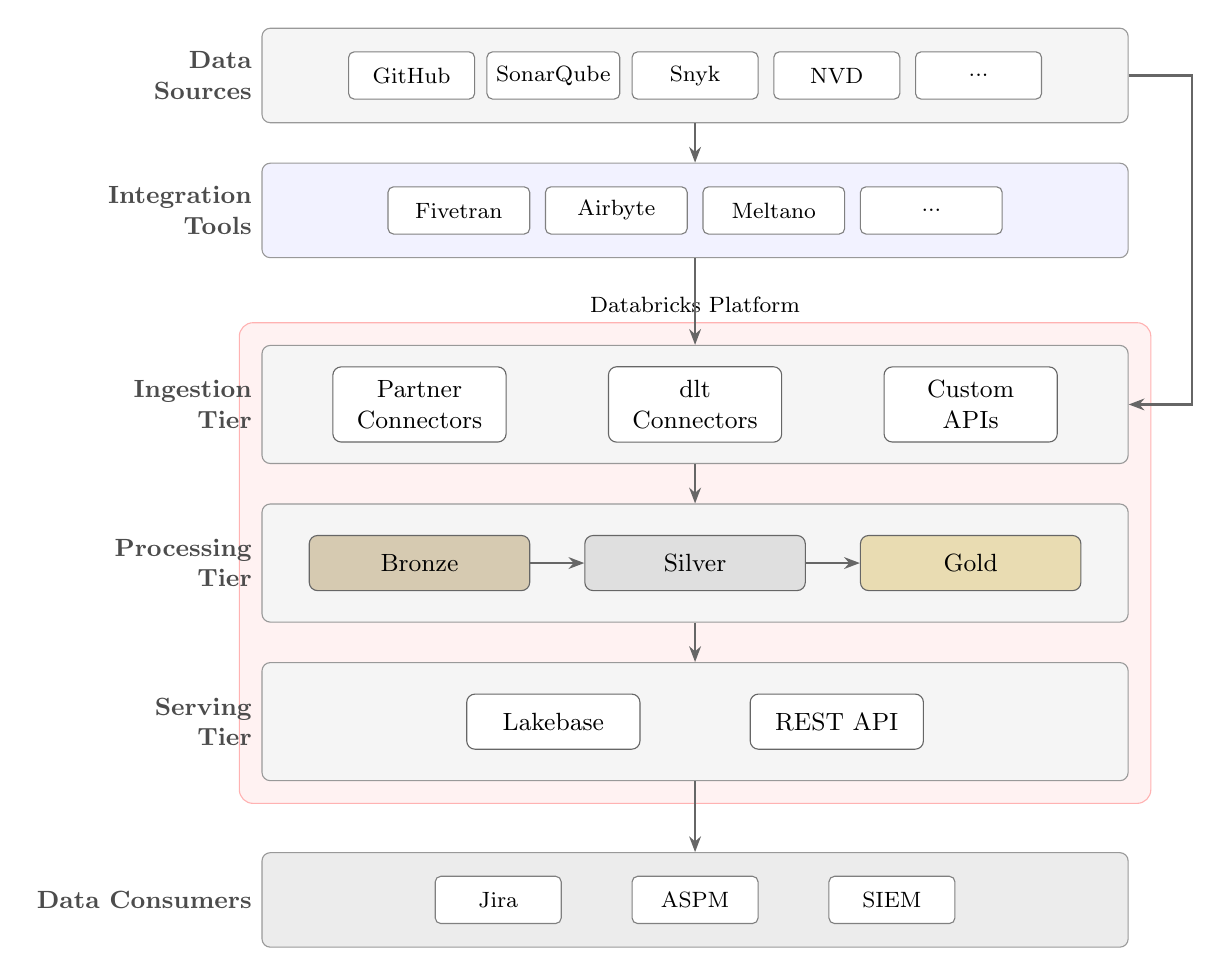
\begin{tikzpicture}[
    node distance=0.5cm,
    tier/.style={rectangle, draw=black!40, fill=gray!8, minimum width=11cm, minimum height=1.2cm, rounded corners=3pt},
    tierbox/.style={rectangle, draw=black!60, fill=white, minimum width=2.2cm, minimum height=0.7cm, font=\small, inner sep=5pt, rounded corners=3pt},
    sourcebox/.style={rectangle, draw=black!50, fill=white, minimum width=1.6cm, minimum height=0.6cm, font=\footnotesize, rounded corners=2pt},
    extbox/.style={rectangle, draw=black!50, fill=white, minimum width=1.8cm, minimum height=0.6cm, font=\footnotesize, rounded corners=2pt},
    consumer/.style={rectangle, draw=black!50, fill=gray!15, minimum width=1.6cm, minimum height=0.6cm, font=\footnotesize, rounded corners=2pt},
    arrow/.style={-{Stealth[length=2mm]}, thick, black!60},
    tierlabel/.style={font=\small\bfseries, text=black!70},
    bronze/.style={fill={rgb,255:red,159;green,122;blue,52}, fill opacity=0.35, text=black, text opacity=1},
    silver/.style={fill={rgb,255:red,192;green,192;blue,192}, fill opacity=0.4, text=black, text opacity=1},
    gold/.style={fill={rgb,255:red,212;green,175;blue,55}, fill opacity=0.35, text=black, text opacity=1},
]

% === DATA SOURCES TIER ===
\node[tier] (sources-bg) {};
\node[tierlabel, left, align=right] at (sources-bg.west) {Data\\Sources};
\node[sourcebox] at ($(sources-bg.center) + (-3.6cm,0)$) (github) {GitHub};
\node[sourcebox] at ($(sources-bg.center) + (-1.8cm,0)$) (sonar) {SonarQube};
\node[sourcebox] at ($(sources-bg.center) + (0,0)$) (snyk) {Snyk};
\node[sourcebox] at ($(sources-bg.center) + (1.8cm,0)$) (nvd) {NVD};
\node[sourcebox] at ($(sources-bg.center) + (3.6cm,0)$) (other) {...};

% === EXTERNAL INTEGRATION TOOLS TIER ===
\node[tier, below=0.5cm of sources-bg, fill=blue!5] (external-bg) {};
\node[tierlabel, left, align=right] at (external-bg.west) {Integration\\Tools};
\node[extbox] at ($(external-bg.center) + (-3cm,0)$) (fivetran) {Fivetran};
\node[extbox] at ($(external-bg.center) + (-1cm,0)$) (airbyte) {Airbyte};
\node[extbox] at ($(external-bg.center) + (1cm,0)$) (meltano) {Meltano};
\node[extbox] at ($(external-bg.center) + (3cm,0)$) (custom) {...};

% === DATABRICKS PLATFORM ===
% Ingestion Tier
\node[tier, below=1.1cm of external-bg, minimum height=1.5cm] (ingestion-bg) {};
\node[tierlabel, left, align=right] at (ingestion-bg.west) {Ingestion\\Tier};
\node[tierbox, align=center] at ($(ingestion-bg.center) + (-3.5cm,0)$) (partner-conn) {Partner\\Connectors};
\node[tierbox, align=center] at ($(ingestion-bg.center) + (0,0)$) (dlt-conn) {dlt\\Connectors};
\node[tierbox, align=center] at ($(ingestion-bg.center) + (3.5cm,0)$) (custom-api) {Custom\\APIs};

% Processing Tier
\node[tier, below=0.5cm of ingestion-bg, minimum height=1.5cm] (processing-bg) {};
\node[tierlabel, left, align=right] at (processing-bg.west) {Processing\\Tier};
\node[tierbox, bronze, minimum width=2.8cm] at ($(processing-bg.center) + (-3.5cm,0)$) (bronze) {Bronze};
\node[tierbox, silver, minimum width=2.8cm] at (processing-bg.center) (silver) {Silver};
\node[tierbox, gold, minimum width=2.8cm] at ($(processing-bg.center) + (3.5cm,0)$) (gold) {Gold};

% Serving Tier
\node[tier, below=0.5cm of processing-bg, minimum height=1.5cm] (serving-bg) {};
\node[tierlabel, left, align=right] at (serving-bg.west) {Serving\\Tier};
\node[tierbox] at ($(serving-bg.center) + (-1.8cm,0)$) (lakebase) {Lakebase};
\node[tierbox] at ($(serving-bg.center) + (1.8cm,0)$) (restapi) {REST API};

% === DATA CONSUMERS ===
\node[tier, below=0.9cm of serving-bg, fill=gray!15] (consumers-bg) {};
\node[tierlabel, left] at (consumers-bg.west) {Data Consumers};
\node[consumer, fill=white] at ($(consumers-bg.center) + (-2.5cm,0)$) (jira) {Jira};
\node[consumer, fill=white] at ($(consumers-bg.center) + (0,0)$) (aspm) {ASPM};
\node[consumer, fill=white] at ($(consumers-bg.center) + (2.5cm,0)$) (siem) {SIEM};

% === ARROWS ===
% Sources to External Tools
\draw[arrow] (sources-bg.south) -- (external-bg.north);

% External Tools to Ingestion
\draw[arrow] (external-bg.south) -- (ingestion-bg.north);

% Direct bypass arrow (Sources to Ingestion) - goes outside on the right
\draw[arrow] (sources-bg.east) -- ++(0.8cm,0) -- ($(ingestion-bg.east) + (0.8cm,0)$) -- (ingestion-bg.east);

% Ingestion to Processing
\draw[arrow] (ingestion-bg.south) -- (processing-bg.north);

% Processing flow
\draw[arrow] (bronze.east) -- (silver.west);
\draw[arrow] (silver.east) -- (gold.west);

% Processing to Serving
\draw[arrow] (processing-bg.south) -- (serving-bg.north);

% Serving to Consumers
\draw[arrow] (serving-bg.south) -- (consumers-bg.north);

% === DATABRICKS BOUNDARY ===
\begin{scope}[on background layer]
\node[draw=red!30, fill=red!5, rounded corners=5pt, fit=(ingestion-bg)(processing-bg)(serving-bg), inner sep=8pt, label={[font=\footnotesize, text=black]above:Databricks Platform}] {};
\end{scope}

\end{tikzpicture}
\caption{Component Design}
\label{fig:component-design}
\end{figure}


\textbf{Data sources} are the external systems analyzed in \autoref{ch:analysis}: application inventories, \gls{scm} platforms, \gls{cicd} tools, security scanners, and vulnerability databases. They are outside the framework's boundary; the framework consumes their \glspl{api} but does not control them.

\textbf{The ingestion tier} hosts connectors that extract data from sources and land it in the bronze layer. Three connector categories serve different integration scenarios. LakeFlow Connect connectors use the platform's managed ingestion service for declarative, zero-code extraction. \gls{sdk} connectors use source-provided client libraries for programmatic extraction with built-in authentication and pagination. \gls{rest} \gls{api} connectors use the open-source \gls{dltool} library for sources that lack a dedicated \gls{sdk}. All connectors share common concerns: authentication, pagination, rate limiting, and incremental state management. The connector framework in \autoref{sec:connector-framework} defines these patterns.

\textbf{The processing tier} implements the medallion architecture (\autoref{sec:medallion-arch}). Delta Lake provides the storage layer; \gls{dltables} orchestrates the transformations. Bronze stores raw ingested data in source-native schemas. Silver normalizes it into the vendor-agnostic entity and finding model defined in \autoref{sec:data-entities}. Gold computes aggregated metrics, \gls{ml}-enriched scores, and consumption-ready datasets. Unity Catalog governs access and tracks lineage across all three layers.

\textbf{The serving tier} exposes processed data to downstream consumers. \gls{sql} warehouses serve \gls{olap} queries for dashboards and analytics. Lakebase serves \gls{oltp} workloads: low-latency lookups, issue tracker integration, and operational \glspl{api}. A \gls{rest} \gls{api} layer provides \gls{http} access to the \gls{oltp} store.

\textbf{Data consumers} are external systems that read from the serving tier: issue trackers (Jira, ServiceNow), \gls{aspm} dashboards, \gls{siem}/\gls{soar} platforms, and custom reporting tools. Like data sources, consumers are outside the framework boundary.

%%% 2.1.3 %%%

\subsection{Medallion Architecture}
\label{sec:medallion-arch}

The processing tier applies the medallion architecture pattern introduced in \autoref{sec:data-architecture}. Each layer is implemented as a Delta Lake schema within a single Unity Catalog, providing unified governance and cross-layer lineage tracking. \autoref{fig:medallion-design} illustrates the layer structure and the transformations between them.

\begin{figure}[htbp]
\centering
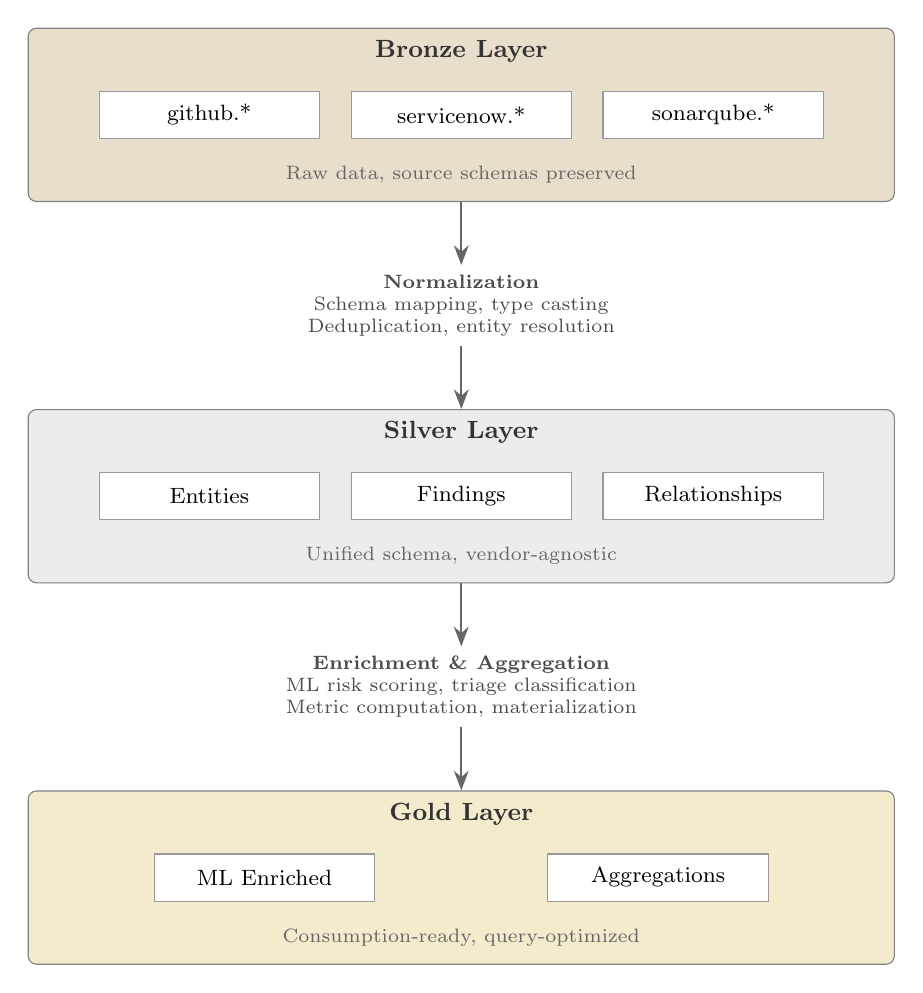
\begin{tikzpicture}[
    node distance=1cm,
    layer/.style={rectangle, draw=black!50, minimum width=11cm, minimum height=2.2cm, rounded corners=3pt},
    schemabox/.style={rectangle, draw=black!40, fill=white, minimum width=2.8cm, minimum height=0.6cm, font=\footnotesize},
    arrow/.style={-{Stealth[length=2.5mm]}, thick, black!60},
    transformation/.style={font=\scriptsize, text=black!70, align=center},
    layerlabel/.style={font=\small\bfseries, text=black!80},
    bronze/.style={fill={rgb,255:red,159;green,122;blue,52}, fill opacity=0.25},
    silver/.style={fill={rgb,255:red,192;green,192;blue,192}, fill opacity=0.3},
    gold/.style={fill={rgb,255:red,212;green,175;blue,55}, fill opacity=0.25},
]

% Bronze Layer
\node[layer, bronze] (bronze-bg) {};
\node[layerlabel] at ($(bronze-bg.north) + (0,-0.3)$) {Bronze Layer};
\node[schemabox] at ($(bronze-bg.center) + (-3.2cm,0)$) {github.*};
\node[schemabox] at ($(bronze-bg.center) + (0,0)$) {servicenow.*};
\node[schemabox] at ($(bronze-bg.center) + (3.2cm,0)$) {sonarqube.*};
\node[font=\scriptsize, text=black!60] at ($(bronze-bg.south) + (0,0.35)$) {Raw data, source schemas preserved};

% Bronze to Silver transformation
\node[transformation, below=0.8cm of bronze-bg] (b2s) {
    \textbf{Normalization}\\
    Schema mapping, type casting\\
    Deduplication, entity resolution
};

% Silver Layer
\node[layer, silver, below=0.8cm of b2s] (silver-bg) {};
\node[layerlabel] at ($(silver-bg.north) + (0,-0.3)$) {Silver Layer};
\node[schemabox] at ($(silver-bg.center) + (-3.2cm,0)$) {Entities};
\node[schemabox] at ($(silver-bg.center) + (0,0)$) {Findings};
\node[schemabox] at ($(silver-bg.center) + (3.2cm,0)$) {Relationships};
\node[font=\scriptsize, text=black!60] at ($(silver-bg.south) + (0,0.35)$) {Unified schema, vendor-agnostic};

% Silver to Gold transformation
\node[transformation, below=0.8cm of silver-bg] (s2g) {
    \textbf{Enrichment \& Aggregation}\\
    ML risk scoring, triage classification\\
    Metric computation, materialization
};

% Gold Layer
\node[layer, gold, below=0.8cm of s2g] (gold-bg) {};
\node[layerlabel] at ($(gold-bg.north) + (0,-0.3)$) {Gold Layer};
\node[schemabox] at ($(gold-bg.center) + (-2.5cm,0)$) {ML Enriched};
\node[schemabox] at ($(gold-bg.center) + (2.5cm,0)$) {Aggregations};
\node[font=\scriptsize, text=black!60] at ($(gold-bg.south) + (0,0.35)$) {Consumption-ready, query-optimized};

% Arrows
\draw[arrow] (bronze-bg.south) -- (b2s.north);
\draw[arrow] (b2s.south) -- (silver-bg.north);
\draw[arrow] (silver-bg.south) -- (s2g.north);
\draw[arrow] (s2g.south) -- (gold-bg.north);

\end{tikzpicture}
\caption{Medallion Layer Design}
\label{fig:medallion-design}
\end{figure}

\subsubsection{Bronze Layer}

The bronze layer stores raw data from each source system with minimal transformation. Each connector writes to its own schema (e.g., \texttt{github}, \texttt{servicenow}, \texttt{sonarqube}), preserving the source's native data structure. Records are appended with standard metadata columns: ingestion timestamp, source system identifier, and batch identifier. No business logic is applied at this layer; the goal is a faithful, auditable copy of source data.

Bronze tables use a schema-on-read approach. New fields from source \gls{api} changes are absorbed through additive schema evolution without breaking existing pipelines. Partitioning by ingestion date enables efficient time-range queries and supports retention policies. Records that fail structural validation at ingestion (malformed \gls{json}, missing required fields) are routed to per-source quarantine tables with diagnostic metadata.

\subsubsection{Silver Layer}

The silver layer is the system of record. Bronze-to-silver transformations normalize heterogeneous source data into the vendor-agnostic domain model defined in \autoref{sec:data-entities}. Three table categories occupy this layer:

\begin{itemize}
    \item \textbf{Entity tables} store normalized dimension data: applications, repositories, teams, commits, pull requests, pipeline runs, dependencies, and branch protection policies. Each entity table uses a surrogate key, a natural key from the source system, and \texttt{valid\_from}/\texttt{valid\_to} timestamps for change tracking.
    \item \textbf{Finding tables} store normalized security findings as fact records. Each finding carries a severity mapped to the canonical scale, a lifecycle status, the source tool identifier, and references to the affected entity (repository, application). Finding tables are organized by category: \gls{sast}, \gls{sca}, secrets, \gls{dast}, containers, and \gls{iac}.
    \item \textbf{Relationship tables} store many-to-many mappings: application-to-repository, finding-to-\gls{cve}, and cross-tool deduplication links.
\end{itemize}

The silver layer applies the data quality patterns from \autoref{sec:data-integration-patterns}: severity harmonization, entity normalization, timestamp standardization, and deduplication. \Gls{dltables} expectations enforce constraints declaratively; records that violate expectations are quarantined rather than propagated.

\subsubsection{Gold Layer}

The gold layer computes consumption-ready datasets from silver data. Two categories of gold tables serve distinct purposes:

\begin{itemize}
    \item \textbf{Aggregation tables} compute metrics at defined grains: application risk scores, team remediation rates, \gls{mttr} by severity, \gls{sla} compliance percentages, and time-series trend roll-ups. These tables power the dashboards and executive reports consumed through the \gls{olap} serving path.
    \item \textbf{\gls{ml}-enriched tables} store model outputs: composite risk scores, false positive predictions, and remediation time estimates. These scores augment the aggregation tables with predictive signals. The \gls{ml} workflow patterns are detailed in \autoref{sec:analytics-patterns}.
\end{itemize}

Gold tables use incremental refresh where possible: new silver records trigger recomputation of only the affected aggregation partitions. Full refresh is reserved for metrics that require global recomputation, such as cross-application percentile rankings.

%%%%%%%%%%%
%%% 2.2 %%%
%%%%%%%%%%%

\section{Data Model}
\label{sec:data-model}

This section maps the conceptual domain model from \autoref{sec:data-entities} to physical table designs across the three medallion layers. It defines reusable schema patterns first, then applies them to produce the concrete entity, finding, and aggregation tables the framework provides.

%%% 2.2.1 %%%

\subsection{Schema Patterns}
\label{sec:schema-patterns}

Schema patterns are reusable templates that standardize how tables are created at each medallion layer. They ensure consistency across the data model and lower the barrier for extending it with new entities or sources. Four patterns cover the framework's needs.

\subsubsection{Bronze Pattern}

Every bronze table follows the same structural convention. The source's native payload is stored alongside a fixed set of metadata columns:

\begin{itemize}
    \item \texttt{\_ingestion\_timestamp} — when the record was ingested (\gls{utc}).
    \item \texttt{\_source\_system} — identifier of the originating tool or platform.
    \item \texttt{\_batch\_id} — unique identifier for the ingestion run, supporting idempotent replays.
    \item \texttt{\_raw\_payload} — the original \gls{json} response or record, preserved for auditability.
\end{itemize}

Additional columns from the source's native schema are included alongside the raw payload through schema-on-read. New fields are absorbed via additive schema evolution. Tables are partitioned by ingestion date to support retention policies and efficient time-range queries.

\subsubsection{Silver Entity Pattern}

Entity tables store normalized dimension data. Each follows a standard structure:

\begin{itemize}
    \item \texttt{id} — surrogate key (auto-generated).
    \item \texttt{natural\_key} — the identifier from the source system (e.g., repository full name, application \texttt{sys\_id}).
    \item \texttt{source\_system} — which tool or platform provided the record.
    \item \texttt{valid\_from} / \texttt{valid\_to} — timestamps for change tracking (Type~2 slowly changing dimension). A \texttt{NULL} value in \texttt{valid\_to} indicates the current version.
    \item Domain-specific columns — attributes defined by the entity type (e.g., \texttt{criticality\_tier} for applications, \texttt{primary\_language} for repositories).
\end{itemize}

The natural key plus source system combination uniquely identifies a record's origin. The surrogate key provides a stable reference for foreign keys even when source identifiers change.

\subsubsection{Silver Finding Pattern}

Finding tables store normalized fact data. Each follows a standard structure:

\begin{itemize}
    \item \texttt{finding\_id} — surrogate key.
    \item \texttt{source\_finding\_id} — the identifier from the source tool.
    \item \texttt{source\_tool} — which scanner produced the finding.
    \item \texttt{repository\_id} — foreign key to the repository entity table.
    \item \texttt{severity} — normalized to the canonical four-level scale (critical, high, medium, low).
    \item \texttt{status} — normalized lifecycle state (open, confirmed, resolved, false\_positive, wontfix).
    \item \texttt{detected\_at} / \texttt{resolved\_at} — \gls{utc} timestamps enabling \gls{mttr} calculation.
    \item \texttt{rule\_id} — the tool-specific rule or check that triggered the finding.
    \item Category-specific columns — attributes unique to the finding type (e.g., \texttt{file\_path} and \texttt{line\_range} for \gls{sast}, \texttt{package\_name} and \texttt{installed\_version} for \gls{sca}).
\end{itemize}

\subsubsection{Relationship Pattern}

Relationship tables store many-to-many mappings between entities. Each contains foreign keys to both sides, a source system indicator, and \texttt{valid\_from}/\texttt{valid\_to} timestamps to track when the relationship was active. No payload columns are included; the table's sole purpose is to link entities. Examples include application-to-repository, finding-to-\gls{cve}, and cross-tool deduplication links.

\subsubsection{Gold Aggregation Pattern}

Aggregation tables follow a grain-metric-period structure:

\begin{itemize}
    \item \textbf{Grain columns} define the level of detail: the entity key (application, team, repository) and time period (day, week, month).
    \item \textbf{Metric columns} store computed values: finding counts by severity, \gls{mttr}, \gls{sla} compliance percentage, risk score.
    \item \textbf{Period columns} store the time window: \texttt{period\_start} and \texttt{period\_end} (\gls{utc}).
    \item \textbf{Refresh metadata}: \texttt{computed\_at} timestamp and refresh strategy indicator (incremental or full).
\end{itemize}

This structure enables consistent querying across all gold tables: filter by grain, aggregate over periods, compare across entities.

%%% 2.2.2 %%%

\subsection{Entity Model}
\label{sec:entity-model}

The silver layer instantiates the schema patterns into concrete tables. This subsection specifies the key tables organized by category: entities (dimensions), findings (facts), reference data, and relationships.

\subsubsection{Entity Tables}

\autoref{tab:entity-tables} lists the entity tables and their key domain-specific columns. All tables include the standard silver entity pattern columns (\texttt{id}, \texttt{natural\_key}, \texttt{source\_system}, \texttt{valid\_from}/\texttt{valid\_to}).

\begin{table}[htbp]
\centering
\caption{Silver Entity Tables}
\label{tab:entity-tables}
\begin{tabularx}{\textwidth}{l l X}
\toprule
\textbf{Table} & \textbf{Source} & \textbf{Key Domain Columns} \\
\midrule
applications & \gls{cmdb} & name, criticality\_tier, lifecycle\_status, business\_unit, compliance\_scope \\
repositories & \gls{scm} & full\_name, primary\_language, visibility, default\_branch, archived, last\_activity\_at \\
teams & \gls{cmdb}/\gls{scm} & name, parent\_team\_id, contact\_email \\
commits & \gls{scm} & sha, author, authored\_at, message, repository\_id \\
pull\_requests & \gls{scm} & number, title, state, author, created\_at, merged\_at, repository\_id \\
pipeline\_runs & \gls{cicd} & pipeline\_id, commit\_sha, status, started\_at, finished\_at, repository\_id \\
dependencies & \gls{sca} & package\_name, installed\_version, license, ecosystem, repository\_id \\
branch\_policies & \gls{scm} & required\_reviewers, require\_status\_checks, enforce\_admins, repository\_id \\
\bottomrule
\end{tabularx}
\end{table}

\subsubsection{Finding Tables}

Finding tables share the silver finding pattern columns and add category-specific attributes. \autoref{tab:finding-tables} summarizes each.

\begin{table}[htbp]
\centering
\caption{Silver Finding Tables}
\label{tab:finding-tables}
\begin{tabularx}{\textwidth}{l X}
\toprule
\textbf{Table} & \textbf{Category-Specific Columns} \\
\midrule
sast\_findings & file\_path, line\_start, line\_end, cwe\_id, language \\
sca\_findings & package\_name, installed\_version, fixed\_version, cve\_id, ecosystem \\
secret\_findings & secret\_type, file\_path, commit\_sha, validity\_status \\
dast\_findings & url, http\_method, parameter, attack\_type \\
container\_findings & image\_name, image\_tag, layer, cve\_id \\
iac\_findings & resource\_type, resource\_name, file\_path, policy\_id, benchmark \\
\bottomrule
\end{tabularx}
\end{table}

Each finding table references its repository through \texttt{repository\_id}. Business application context is derived through the relationship tables rather than stored directly on findings, preserving the many-to-many application-to-repository mapping without duplicating finding records.

\subsubsection{Reference Tables}

Reference tables store external intelligence used for enrichment:

\begin{itemize}
    \item \textbf{vulnerabilities} — \gls{cve} records with description, published date, and \gls{cvss} base score from the \gls{nvd}.
    \item \textbf{epss\_scores} — daily \gls{epss} probabilities per \gls{cve}, enabling time-series analysis of exploitation likelihood.
    \item \textbf{kev\_entries} — \gls{cisa} \gls{kev} catalog entries indicating confirmed active exploitation, with the date added.
\end{itemize}

These tables are refreshed on a scheduled basis from their respective external sources. Findings link to them through \gls{cve} identifiers, forming the three-signal enrichment model described in \autoref{sec:static-appsec}.

\subsubsection{Relationship Tables}

Three relationship tables implement the key mappings identified in the domain model:

\begin{itemize}
    \item \textbf{app\_repo\_mapping} — links applications to repositories (many-to-many). This is the most critical relationship for business context attribution.
    \item \textbf{finding\_cve\_mapping} — links findings to \gls{cve} records, enabling vulnerability enrichment.
    \item \textbf{dedup\_links} — links findings identified as duplicates across tools, preserving traceability to each source report while establishing a canonical finding.
\end{itemize}

%%% 2.2.3 %%%

\subsection{Aggregation Model}
\label{sec:aggregation-model}

The gold layer computes consumption-ready metrics from silver data using the aggregation pattern. Each gold table targets a specific stakeholder need identified in \autoref{sec:data-entities}.

\subsubsection{Application Risk Scores}

The \texttt{app\_risk\_scores} table computes a composite risk metric per application per period. Grain columns are \texttt{application\_id} and time period. Metric columns include: open finding counts by severity, weighted risk score (combining severity, \gls{epss} probability, and application criticality tier), \gls{sla} compliance percentage, and a trend indicator (improving, stable, degrading). This table serves application owners who need a single view of their application's security posture.

\subsubsection{Team Metrics}

The \texttt{team\_metrics} table aggregates remediation performance per team per period. Metrics include: \gls{mttr} by severity, finding closure rate, new vs. resolved finding ratio, and \gls{sla} breach count. Leadership uses these metrics for cross-team comparisons and resource allocation decisions.

\subsubsection{Vulnerability Trends}

The \texttt{vulnerability\_trends} table provides time-series data at configurable grains (daily, weekly, monthly). Metrics include: new findings introduced, findings resolved, net open count, severity distribution shifts, and mean age of open findings. These trends power the longitudinal dashboards that track organizational progress.

\subsubsection{Coverage Analysis}

The \texttt{coverage\_analysis} table identifies gaps in security tool coverage. For each repository, it records which tool categories have produced findings or scan records (indicating active scanning) and which have not. Missing coverage is flagged per category: a repository with no \gls{sast} findings and no \gls{sast} pipeline runs likely lacks static analysis integration. This table enables security teams to prioritize tooling rollout.

\subsubsection{Extension Guide}

Adding a new gold table follows a consistent process: define the grain (which entity, which time period), specify the metrics (what to compute), write a silver-to-gold \gls{dltables} transformation, and configure the refresh strategy (incremental or full). The aggregation pattern ensures all gold tables share a common query interface, so dashboards and reporting tools can consume new tables without structural changes.

%%%%%%%%%%%
%%% 2.3 %%%
%%%%%%%%%%%

\section{Environment and Deployment}
\label{sec:env-deploy}

The solution architecture (\autoref{sec:solution-arch}) and data model (\autoref{sec:data-model}) define the framework's components and data structures. Before these can be populated with connectors or analytics, the deployment environment must be provisioned and the codebase organized. This section covers the foundational setup: deployment strategy, project structure, pipeline orchestration, monitoring, and deployment-level verification. These are one-time decisions that establish the platform; the repeatable patterns for extending the framework with new sources and analytics follow in \autoref{sec:connector-framework} and \autoref{sec:analytics-serving}.

%%% 2.3.1 %%%

\subsection{Deployment Strategy}
\label{sec:deployment-strategy}

The framework uses Databricks Asset Bundles as its deployment mechanism~\cite{DatabricksDAB2025}. A bundle is a declarative configuration that describes Databricks resources (jobs, pipelines, cluster policies, permissions) alongside the source code that implements them. A single \texttt{databricks.yml} configuration file at the project root defines all resource mappings, inter-resource dependencies, and environment-specific parameter overrides. This approach treats the deployment as \gls{iac}: the entire platform configuration is version-controlled, reviewable, and reproducible from a single source.

Three environment targets structure the promotion path: development, staging, and production. Each target overrides a set of parameters: the Unity Catalog catalog name (one catalog per environment, following the namespace design from \autoref{sec:tech-stack}), compute cluster sizing, permission grants, and pipeline scheduling intervals. Development uses smaller clusters and relaxed permissions for rapid iteration. Staging mirrors production configuration for pre-release validation. Production enforces strict access controls, full-scale compute, and scheduled execution.

A \gls{cicd} pipeline automates the build-test-deploy cycle~\cite{DatabricksCICD2025}. On each code change, the pipeline executes three stages: validation checks bundle configuration syntax and resource compatibility, testing runs the project's test suite against the development environment, and deployment promotes the validated bundle to the target environment. Staging and production deployments require an approval gate; only reviewed and tested changes reach shared environments. The pipeline runs on standard \gls{cicd} platforms (GitHub Actions, Azure DevOps, GitLab \gls{cicd}) that invoke the Databricks \gls{cli} for bundle operations.

%%% 2.3.2 %%%

\subsection{Project Structure}
\label{sec:project-structure}

The project follows a monorepo layout: all connectors, transformations, analytics, tests, and deployment configuration reside in a single repository. This simplifies dependency management, enables atomic cross-layer changes, and supports the bundle deployment model described in \autoref{sec:deployment-strategy}. The repository organizes into four top-level directories: \texttt{src/} for pipeline source code (connectors, transformations, analytics), \texttt{tests/} for the test suite, \texttt{config/} for lookup tables and environment-specific settings, and the bundle configuration files at the root.

Within \texttt{src/}, each connector is an independent module containing its own ingestion and transformation logic. Shared utilities (authentication helpers, pagination handlers, normalization functions) reside in a common library that connectors import. Silver-to-gold transformations are grouped by analytic rather than by source, since a single gold table may consume data from multiple connectors. This boundary ensures that adding a new connector requires changes only within its own module and the relevant gold-layer pipelines.

Naming conventions enforce consistency across the platform. Unity Catalog objects follow the pattern \texttt{<env>.<layer>\_<source>.<table\_name>}: for example, \texttt{prod.bronze\_github.code\_scanning\_alerts} or \texttt{prod.silver.sast\_findings}. Pipeline names mirror their source module: \texttt{ingest\_github}, \texttt{transform\_github\_silver}. Column names use \texttt{snake\_case} throughout. These conventions reduce cognitive load and simplify governance policies that rely on name-based access rules.

Configuration management separates secrets from non-sensitive settings. Secrets (\gls{api} tokens, service account credentials) are stored in the platform's secret scope and referenced by name in pipeline code; they never appear in source files or bundle configuration. Non-sensitive settings (severity mapping tables, \gls{sla} thresholds, scheduling intervals) are version-controlled as configuration files and loaded at pipeline runtime. Environment-specific overrides in the bundle configuration select the appropriate catalog, secret scope, and compute target for each deployment.

%%% 2.3.3 %%%

\subsection{Pipeline Orchestration}
\label{sec:orchestration}

Lakeflow Jobs is the orchestration engine that schedules and coordinates pipeline execution~\cite{DatabricksLakeflowJobs2026}. A job groups related tasks into a \gls{dag} with explicit dependencies; the engine executes tasks in dependency order and handles retries on failure. Jobs are defined in the bundle configuration alongside the resources they operate on, making orchestration version-controlled and promotable across environments through the same deployment path described in \autoref{sec:deployment-strategy}.

The framework assigns one job per connector. Each connector job contains two sequential tasks: an ingestion task that extracts data from the source \gls{api} into bronze, and a transformation task that normalizes bronze records into silver. This isolation gives each connector an independent failure domain: a GitHub \gls{api} outage does not block ServiceNow ingestion. Gold-layer analytics run as separate jobs that list their upstream connector jobs as dependencies; the orchestrator starts a gold job only after all required silver data is fresh. \gls{ml} model retraining runs on independent schedules, decoupled from the ingestion cycle.

Source characteristics drive scheduling frequency. High-change sources (\gls{scm} platforms, security scanners producing frequent new findings) run on shorter intervals, typically hourly. Stable sources (application inventory from the \gls{cmdb}) run daily. External enrichment sources follow their respective update cadences: \gls{nvd} and \gls{epss} update daily, \gls{cisa} \gls{kev} updates on weekdays. Gold analytics trigger after their upstream connector jobs complete through explicit job dependencies. Where strict ordering adds unnecessary complexity, such as daily reporting workloads, a schedule offset from the expected ingestion window is an acceptable alternative.

Each task is configured with a retry count and backoff interval for transient failures. If retries exhaust, the task fails and downstream tasks within the same job do not execute. Job-level alerts notify operators of persistent failures through configured channels (email, messaging webhooks). Since connector jobs are independent, a single connector degradation does not cascade. Jobs run in parallel on ephemeral job clusters that are created at job start and terminated at completion, preventing resource contention between connectors and ensuring cost efficiency through right-sized compute per workload.

%%% 2.3.4 %%%

\subsection{Monitoring and Observability}
\label{sec:monitoring}

Orchestration ensures pipelines run on schedule; monitoring ensures they run correctly over time. The platform provides system tables that record job execution history, pipeline events, and compute utilization~\cite{DatabricksObservability2026}. The framework builds on these tables to track three dimensions: data freshness, pipeline health, and data quality trends. All monitoring queries run against the same \gls{sql} warehouse that serves analytics, keeping the operational overhead within the platform.

Data freshness tracks the recency of data at each medallion layer. Each bronze table records the timestamp of its last successful ingestion; each silver table records its last transformation run. A freshness monitor queries these timestamps and flags tables where the age exceeds a configurable threshold. Thresholds reflect the scheduling frequency from \autoref{sec:orchestration}: an hourly connector that has not produced data in two hours is stale; a daily enrichment source that has not refreshed in 36 hours is stale. Freshness violations trigger alerts through the same channels configured for job failures.

Pipeline health aggregates job execution metrics from system tables. Key indicators include: job success rate over a rolling window, mean run duration and its trend (detecting performance degradation before it causes timeouts), task-level retry frequency (high retry rates signal intermittent source issues), and quarantine volume (records routed to quarantine tables per ingestion run). A rising quarantine rate often precedes data quality issues in the silver layer and warrants investigation before downstream aggregations are affected.

Alerting bridges monitoring signals to operational response. The framework configures alerts at two levels. Job-level alerts fire on individual failures or threshold breaches, such as a quarantine rate exceeding a configured percentage of ingested records. System-level alerts fire on aggregate degradation: multiple connectors stale simultaneously, overall pipeline success rate below a threshold, or gold tables not refreshed within their expected window. Alerts are delivered through configured channels (email, messaging webhooks, incident management integrations). The thresholds and channels are defined as configuration, not code, enabling operators to tune sensitivity without redeploying pipelines.

%%% 2.3.5 %%%

\subsection{Testing and Validation}
\label{sec:env-testing}

This subsection covers deployment-level verification: the checks that confirm the environment is correctly provisioned and the codebase meets quality standards. Component-level testing patterns for connectors and analytics are defined separately in \autoref{sec:connector-testing} and \autoref{sec:analytics-testing}.

The \gls{cicd} pipeline enforces quality gates before deployment. Linting validates code style and catches common errors (unused imports, undefined variables, type mismatches). Formatting ensures consistent code layout across contributors. Unit tests verify individual functions (severity mapping lookups, timestamp parsers, schema mapping logic) in isolation from the platform. All gates must pass before the pipeline proceeds to deployment.

After deployment, environment validation confirms that infrastructure prerequisites are in place. Automated checks verify that Unity Catalog objects (catalogs, schemas, tables) exist with expected permissions, compute resources (clusters, \gls{sql} warehouses) are configured and accessible, secret scopes contain the required credentials, and \gls{dltables} pipelines are registered. These checks serve as smoke tests for newly provisioned or updated environments. Failures block pipeline execution until the environment is corrected.

The framework uses pytest markers to link individual tests to requirement identifiers. Each test function carries a marker referencing a specific requirement from \autoref{ch:analysis}, such as \texttt{@pytest.mark.requirement("REQ-SCA-001")}. A traceability matrix is generated automatically from test results, mapping each requirement to its covering tests and their pass/fail status. This pattern applies uniformly across environment, connector (\autoref{sec:connector-testing}), and analytics (\autoref{sec:analytics-testing}) testing. The cross-cutting traceability matrix that summarizes coverage across all components is produced in the reference implementation (\autoref{sec:testing-validation}).

%%%%%%%%%%%
%%% 2.4 %%%
%%%%%%%%%%%

\section{Connector Framework}
\label{sec:connector-framework}

The connector framework defines how data moves from the heterogeneous sources analyzed in \autoref{ch:analysis} into the medallion layers described in \autoref{sec:medallion-arch}. \autoref{sec:component-design} introduced three connector categories (LakeFlow Connect, \gls{sdk}, and \gls{rest} \gls{api} with \gls{dltool}); this section specifies the common abstraction they share, the patterns for landing data in bronze, and the patterns for transforming it to silver. The goal is a repeatable recipe: adding a new source requires implementing a well-defined set of concerns against a new \gls{api}, not redesigning the pipeline.

%%% 2.4.1 %%%

\subsection{Connector Abstraction}
\label{sec:connector-abstraction}

Every connector must handle the same set of cross-cutting concerns, but the three connector categories introduced in \autoref{sec:component-design} differ in how much of this work the developer performs versus the platform or library.

\subsubsection{Connector Categories}

\textbf{LakeFlow Connect connectors} use the platform's managed ingestion service. They are declarative: the connector is configured through the bundle definition, not coded. Authentication, pagination, incremental state, and schema inference are handled by the platform. This category suits sources with supported LakeFlow Connect integrations where full-table ingestion meets requirements. The trade-off is limited flexibility: custom transformation logic, selective field extraction, and non-standard pagination cannot be injected.

\textbf{\gls{sdk} connectors} use a source-provided client library (e.g., the \gls{aws} \gls{sdk} for Python, PyGitHub, python-gitlab) for programmatic extraction. These \glspl{sdk} encapsulate authentication, pagination, rate limiting, and object model mapping, letting the developer work with high-level methods rather than raw \gls{http} requests. This category suits sources that offer an official \gls{sdk} with good coverage of the required endpoints. The developer controls the extraction logic, but the \gls{sdk} handles the transport-level concerns.

\textbf{\gls{rest} \gls{api} connectors with \gls{dltool}} use the open-source \gls{dltool} library to build ingestion pipelines against sources that lack a dedicated \gls{sdk}. The library provides pre-built authentication, pagination, and incremental loading components that the developer composes declaratively against the source's \gls{rest} \gls{api}. This category handles the mechanical concerns (request construction, response parsing, state management) while the developer specifies endpoints, schema mapping, and extraction parameters.

The decision follows a preference order: use LakeFlow Connect if a supported integration exists and meets requirements; use the source's \gls{sdk} when one is available with sufficient endpoint coverage; fall back to \gls{dltool} for sources with only a \gls{rest} \gls{api}. The five responsibilities defined below represent the full contract. \gls{rest} \gls{api} connectors implement them through \gls{dltool} library components. \gls{sdk} connectors delegate them to the client library. LakeFlow Connect connectors satisfy them through platform configuration. The reference implementation in \autoref{ch:implementation} demonstrates all three categories.

\subsubsection{Authentication}

Security tool \glspl{api} use several authentication mechanisms: \glspl{pat}, OAuth~2.0 client credentials, and service account keys. The connector abstraction externalizes credentials through a platform secret scope. Each connector declares which credential type it requires; the framework resolves it at runtime. This separation keeps secrets out of pipeline code and enables credential rotation without redeploying connectors.

\subsubsection{Pagination}

The source integration summary in \autoref{sec:source-integration-summary} shows that \gls{rest} \glspl{api} are the dominant integration surface. These \glspl{api} return results in pages. Two pagination strategies cover the majority of sources: offset-based (page number and size parameters) and cursor-based (an opaque token returned with each response). The connector abstraction encapsulates the pagination strategy so that downstream pipeline logic receives a continuous stream of records regardless of the underlying mechanism. GraphQL-based sources such as the GitHub \gls{api} use cursor-based pagination exclusively.

\subsubsection{Rate Limiting}

Source \glspl{api} enforce rate limits, typically expressed as requests per time window. The connector abstraction implements adaptive backoff: when a rate limit response is received (\gls{http} 429), the connector pauses for the duration specified in the response headers before retrying. For sources without explicit rate limit headers, configurable per-source rate limits prevent exceeding undocumented thresholds. Transient errors (\gls{http} 5xx) trigger exponential backoff with a configurable maximum retry count.

\subsubsection{Incremental State}

Full re-ingestion does not scale for enterprise environments with large data volumes, as discussed in \autoref{sec:data-integration-patterns}. Each connector maintains a high-water mark: the timestamp or cursor of the last successfully ingested record. On subsequent runs, the connector resumes from this position, fetching only new or changed records. The high-water mark is persisted in a state table within the bronze schema, co-located with the data it tracks. For sources that support \gls{cdc} (e.g., ServiceNow's update set mechanism), the connector consumes change events directly.

\subsubsection{Extension Points}

Adding a new source connector follows the category preference order. For a LakeFlow Connect connector: register credentials, add the connector configuration to the bundle definition, and map the landing tables to the bronze schema. For an \gls{sdk} connector: register credentials, implement the extraction logic using the source's client library, define the high-water mark column, and configure the bronze table. For a \gls{rest} \gls{api} connector with \gls{dltool}: register credentials, define the \gls{rest} \gls{api} source configuration (base \gls{url}, endpoints, pagination type), and configure the \gls{dltool} pipeline to land in the bronze schema. In all three cases, no changes to the silver or gold layers are needed at this stage; transformation patterns (\autoref{sec:transformation-patterns}) handle the mapping separately.

%%% 2.4.2 %%%

\subsection{Ingestion Patterns}
\label{sec:ingestion-patterns}

Ingestion moves data from source \glspl{api} into the bronze layer. All connectors follow the same landing pattern, with source-type-specific variations described below.

\subsubsection{Common Landing Pattern}

Every ingestion run produces append-only writes to the target bronze table. The full \gls{api} response is preserved in the \texttt{\_raw\_payload} column alongside the metadata columns defined by the bronze schema pattern (\autoref{sec:schema-patterns}): ingestion timestamp, source system identifier, and batch identifier. No field filtering or transformation occurs at this stage; the bronze layer is a faithful copy of source data.

The batch identifier enables idempotent replays. If a pipeline run fails partway through, re-executing the same batch overwrites only the records from that batch, preventing duplicates. For sources where merge semantics are appropriate (e.g., entity snapshots from a \gls{cmdb}), the connector uses upsert writes keyed on the source record's natural identifier.

Records that fail structural validation at landing, such as malformed \gls{json} or responses with unexpected schema changes, are routed to per-source quarantine tables. Each quarantine record includes the raw payload, the error description, and the batch identifier. This quarantine pattern ensures zero silent data loss: every record retrieved from a source is either successfully landed or isolated with a documented failure reason~\cite{DAMA2017}.

\subsubsection{Source Code Management Sources}

\gls{scm} connectors pull repository metadata, commits, pull requests, and branch protection configurations through \gls{rest} or GraphQL \glspl{api}. These sources produce moderate data volumes with frequent updates. The high-water mark is typically the \texttt{updated\_at} timestamp on the most recently modified record. Webhook-triggered runs complement scheduled pulls for near-real-time ingestion of events such as new pull requests or merged commits.

\subsubsection{Security Scanner Sources}

Security scanner connectors handle the widest format diversity. Server-based tools (SonarQube, Snyk, Dependency-Track) expose \gls{rest} \glspl{api} with paginated \gls{json} responses, similar to \gls{scm} sources. \gls{cli}-based tools (Semgrep, TruffleHog, Trivy) produce output files in \gls{json} or \gls{sarif} format~\cite{OASIS2024} that must be collected from \gls{cicd} pipeline artifacts or uploaded to a staging location. Platform-integrated scanners (GitHub Code Scanning, GitLab Security) expose findings through their host platform's \gls{api}, sharing the same authentication and pagination infrastructure as the \gls{scm} connector for that platform.

For \gls{sarif}-producing tools, the connector preserves the full \gls{sarif} document in the raw payload. \gls{sarif} encodes results, rules, and tool metadata in a single structure, and parsing it into individual findings is deferred to the transformation layer.

\subsubsection{Application Inventory Sources}

\gls{cmdb} connectors differ from other sources in two ways. First, they must traverse relationships: an application record references its owning team, associated repositories, and dependent services through foreign key attributes or relationship tables in the \gls{cmdb}. The connector must resolve these references during ingestion, either by following relationship \glspl{api} or by ingesting related tables separately and joining them in the transformation layer. Second, \gls{cmdb} data includes organization-specific custom attributes (e.g., compliance scope, data classification) that vary across deployments. The schema-on-read approach at the bronze layer absorbs these custom fields without requiring connector changes.

%%% 2.4.3 %%%

\subsection{Transformation Patterns}
\label{sec:transformation-patterns}

Transformations move data from the bronze layer to the silver entity and finding tables defined in \autoref{sec:entity-model}. Each transformation is a \gls{dltables} pipeline that reads from one or more bronze tables and writes to a silver table. Five patterns compose the bronze-to-silver path.

\subsubsection{Schema Mapping}

Each source connector has a corresponding schema mapping that extracts typed columns from the bronze raw payload. The mapping defines which \gls{json} fields correspond to which silver columns, applies type casts (e.g., string timestamps to \gls{utc} datetime), and assigns the surrogate key. Mappings are defined declaratively as column expressions in the \gls{dltables} pipeline, making them easy to review and update when source schemas change.

\subsubsection{Normalization}

Three normalization rules bring heterogeneous source data to a common form:

\begin{itemize}
    \item \textbf{Severity harmonization.} Tools use different severity scales, as described in \autoref{sec:static-appsec}. The framework maps each tool's native scale to the canonical four-level model (critical, high, medium, low) through per-tool lookup tables. These tables are maintained as configuration, not code, enabling updates without pipeline changes.
    \item \textbf{Status normalization.} Finding lifecycle states vary across tools (e.g., SonarQube's ``confirmed'' vs. GitHub's ``open''). A per-tool status mapping translates each tool's states to the canonical five-state model (open, confirmed, resolved, false\_positive, wontfix).
    \item \textbf{Timestamp standardization.} All timestamps are converted to \gls{utc}. Source-specific formats (ISO~8601, Unix epoch, tool-specific strings) are parsed during schema mapping and stored as \gls{utc} datetime columns.
\end{itemize}

\subsubsection{Data Quality Validation}

\Gls{dltables} expectations enforce constraints on every record entering the silver layer. Expectations are declared alongside the transformation logic and checked at runtime. Examples include: severity must be one of the four canonical values, status must be one of the five canonical states, repository foreign keys must reference an existing silver entity, and timestamps must fall within a plausible range. Records that violate expectations are quarantined rather than propagated, consistent with the quarantine pattern applied at ingestion.

\subsubsection{Deduplication}

When multiple tools scan the same repository, overlapping findings must be identified and linked. Three deduplication strategies handle different overlap scenarios:

\begin{itemize}
    \item \textbf{Exact \gls{cve} match.} Two \gls{sca} findings referencing the same \gls{cve} and package in the same repository are duplicates. This is the simplest case.
    \item \textbf{Location-based matching.} Two \gls{sast} findings targeting the same file, line range, and weakness category (mapped via \gls{cwe}) in the same repository are likely duplicates. A confidence threshold accounts for minor line number differences caused by tool-specific parsing.
    \item \textbf{Cross-category correlation.} A secret detected by both a \gls{cli}-based scanner and a platform-integrated scanner at the same file path and commit is a duplicate. Matching uses the secret type and file location.
\end{itemize}

Deduplicated findings are not deleted. Instead, a deduplication link record is created in the \texttt{dedup\_links} relationship table (\autoref{sec:entity-model}), preserving traceability to each source report while establishing a canonical finding for aggregation. Deduplication pairs are enumerated per tool combination in the reference implementation (\autoref{ch:implementation}).

\subsubsection{Business Context Attribution}

The final transformation step links findings to business applications. The \texttt{app\_repo\_mapping} relationship table maps repositories to applications. Since this mapping is many-to-many (one application may span multiple repositories; one repository may serve multiple applications), findings inherit application context through a join rather than a direct foreign key. This join enables the gold-layer aggregations in \autoref{sec:aggregation-model} to compute per-application metrics. The mapping itself is sourced from the \gls{cmdb} connector and can be supplemented by automated repository-to-application inference in the \gls{ml} workflows described in \autoref{sec:analytics-patterns}.

%%% 2.4.4 %%%

\subsection{Testing and Validation}
\label{sec:connector-testing}

Connector tests use the pytest infrastructure and requirement markers established in \autoref{sec:env-testing}. Three additional libraries complete the connector testing stack. An \gls{http} request mocking library (such as \texttt{responses} or \texttt{requests-mock}) intercepts \gls{api} calls to simulate source system behavior without network access. A PySpark DataFrame assertion library (such as \texttt{chispa}) compares transformation outputs against expected results with clear diff reporting. \Gls{dltables} expectations, defined alongside transformation logic, provide runtime data quality validation within pipeline execution. Together, these tools enable isolated, reproducible tests that run in the \gls{cicd} pipeline without depending on live source systems.

Ingestion tests verify the connector abstraction concerns from \autoref{sec:connector-abstraction}. Authentication tests confirm that credentials are resolved from the secret scope and that invalid or expired tokens produce clear error messages rather than silent failures. Pagination tests supply multi-page mock responses and verify that the connector retrieves all pages without data loss or duplication. Rate limit tests simulate \gls{http}~429 responses and verify that the connector pauses and retries according to the backoff policy. Incremental state tests run the connector twice with an intermediate data change and confirm the second run fetches only new records, resuming correctly from the persisted high-water mark. Shared test fixtures provide reusable mock response generators for common \gls{api} patterns.

Transformation tests verify the bronze-to-silver path from \autoref{sec:transformation-patterns}. Schema mapping tests supply known bronze payloads and assert that silver columns have correct types, values, and null handling. Severity normalization tests verify that every value in the tool's native severity scale maps to the correct canonical level; the test dataset must cover all source-specific values, including edge cases such as ``informational'' or ``unknown'' that the tool may produce. Status normalization tests cover all tool-specific lifecycle states similarly. Timestamp tests cover format edge cases: ISO~8601 with and without timezone offsets, Unix epoch in seconds and milliseconds, and tool-specific string formats. Tests are data-driven: each case is a pair of (input bronze record, expected silver record), maintained as \gls{json} fixtures alongside the connector module.

Data quality tests verify \gls{dltables} expectation behavior. For each expectation defined on a silver table, a test supplies a record that violates the constraint and confirms it is routed to the quarantine table. A complementary test supplies a valid record and confirms it passes through. Deduplication tests supply known duplicate pairs (same \gls{cve} and package for \gls{sca}, same file, line range, and \gls{cwe} for \gls{sast}, same file path and commit for secrets) and verify that correct \texttt{dedup\_links} records are created. Negative cases supply similar but distinct findings and verify they are not incorrectly linked.

Every connector must pass tests covering: authentication and credential resolution, pagination across multiple response pages, rate limit backoff, incremental state resume, schema mapping for all ingested endpoints, severity and status normalization for all source-specific values, at least one data quality expectation per silver table, and deduplication for all applicable tool overlap pairs. New connectors are not merged until this suite passes in the \gls{cicd} pipeline.

%%%%%%%%%%%
%%% 2.5 %%%
%%%%%%%%%%%

\section{Analytics and Serving Framework}
\label{sec:analytics-serving}

The data model (\autoref{sec:data-model}) and connector framework (\autoref{sec:connector-framework}) defined how data is structured and ingested. This section addresses the final stage: computing consumption-ready insights from silver data and delivering them to stakeholders. \autoref{sec:aggregation-model} defined \emph{which} gold tables the framework provides; this section defines \emph{how} those computations are structured and how the results reach consumers through analytical, operational, and event-driven channels.

%%% 2.5.1 %%%

\subsection{Analytics Patterns}
\label{sec:analytics-patterns}

Gold-layer computations fall into two categories: rule-based analytics that apply deterministic formulas to silver data, and \gls{ml}-driven analytics that learn patterns from historical data. Both produce outputs that follow the gold aggregation pattern defined in \autoref{sec:schema-patterns}.

\subsubsection{Rule-Based Analytics}

Rule-based analytics implement deterministic business logic as \gls{sql} transformations or \gls{dltables} pipelines. Three computation patterns cover the framework's needs.

\textbf{Composite scoring} combines multiple signals into a single metric. The application risk score, for example, weights open finding counts by severity, multiplies by \gls{epss} exploitation probability, and factors in the application's criticality tier. The formula is configurable: organizations assign weights to each signal based on their risk appetite. \gls{sla} compliance calculations follow the same pattern, comparing finding ages against severity-specific thresholds to produce a compliance percentage.

\textbf{Time-series aggregation} rolls up finding data at daily, weekly, and monthly grains. Each roll-up computes period metrics (new findings, resolved findings, net open count) and derived indicators (period-over-period change, moving averages, severity distribution shifts). These aggregations power the trend dashboards that track organizational progress over time.

\textbf{Threshold classification} assigns categorical labels based on metric values. Risk tiers (critical, high, medium, low) are assigned to applications based on their composite score. Coverage gaps are flagged when a repository lacks scan records for a tool category. \gls{sla} breaches are marked when open finding age exceeds the severity-specific threshold. These classifications enable filtering and alerting in downstream serving.

Two refresh strategies apply to rule-based analytics. \textbf{Incremental refresh} recomputes only the partitions affected by new silver records; this suits most aggregations where each record maps to a single grain partition (e.g., one application, one time period). \textbf{Full refresh} recomputes the entire table; this is necessary for metrics that depend on global state, such as cross-application percentile rankings or organization-wide severity distributions.

\subsubsection{ML-Driven Analytics}

\gls{ml}-driven analytics learn patterns from historical silver and gold data to produce predictive signals that rule-based formulas cannot capture. The framework supports four use cases.

\textbf{Composite risk scoring} predicts which applications carry the highest real risk by combining finding data with development activity signals (commit frequency, dependency age, remediation velocity). Unlike the rule-based risk score that weights predefined signals, the \gls{ml} model learns which combinations of factors historically preceded security incidents.

\textbf{False positive prediction} estimates the probability that a new finding is a false positive, based on patterns in historical triage decisions. Features include the source tool, rule identifier, file type, finding age at triage, and the repository's historical false positive rate for the same rule. High-confidence predictions reduce noise for developers by deprioritizing likely false positives in dashboards and notifications.

\textbf{Remediation time estimation} predicts \gls{mttr} for new findings based on historical resolution data. Features include severity, tool category, repository activity level, team workload, and dependency complexity. These predictions inform \gls{sla} compliance forecasting and resource allocation.

\textbf{Anomaly detection} identifies unusual patterns: unexpected spikes in finding volumes, sudden changes in severity distributions, or new finding categories appearing in previously clean repositories. These signals flag potential tool misconfigurations, new attack surfaces, or integration issues that warrant investigation.

The \gls{ml} workflow uses three platform components. MLflow provides experiment tracking, model versioning, and a model registry that manages the lifecycle from development through staging to production~\cite{MLflow2025}. The Feature Store provides reusable feature tables computed from silver and gold data, ensuring consistent feature definitions across training and inference~\cite{DatabricksFeatureEng2025}. Model Serving exposes registered models as real-time inference endpoints for latency-sensitive predictions.

Model outputs integrate into the gold layer through two paths. Batch predictions (risk scores, false positive probabilities) are written to dedicated columns on gold tables during scheduled pipeline runs, augmenting the rule-based metrics with predictive signals. Real-time predictions (on-demand risk assessments for newly ingested findings) are served through inference endpoints and cached in Lakebase for low-latency access.

\subsubsection{Extension Blueprint}

Adding a new analytics workflow follows a consistent process regardless of type. First, define the business question the analytic answers and identify the stakeholder it serves. Second, determine whether a rule-based formula or an \gls{ml} model is appropriate: rule-based suits well-understood relationships with clear formulas; \gls{ml} suits pattern recognition over complex, high-dimensional data. Third, implement the computation as a \gls{dltables} pipeline (rule-based) or an MLflow-tracked experiment (\gls{ml}). Fourth, wire the output to a gold table following the aggregation pattern, configure the refresh strategy, and register the new table in Unity Catalog for governance and lineage tracking.

%%% 2.5.2 %%%

\subsection{Serving Patterns}
\label{sec:serving-patterns}

The serving layer delivers gold-layer outputs to the data consumers identified in \autoref{sec:component-design}. Three delivery modes address different access patterns and latency requirements.

\subsubsection{Analytical Serving}

Analytical serving targets dashboards, reporting tools, and ad-hoc analysis through the \gls{olap} path. A \gls{sql} warehouse executes queries against gold-layer Delta tables, providing sub-five-second response times for pre-computed aggregations. Materialized views cache frequently accessed query patterns, reducing compute cost for recurring dashboard refreshes.

Stakeholder-specific views organize gold data for each audience: executive risk overviews surface application risk scores and organizational trends, team dashboards present remediation metrics and \gls{sla} compliance, and security engineering views expose tool coverage gaps and deduplication statistics. These views are implemented as \gls{sql} views on top of the gold tables, not separate data copies, ensuring consistency across all consumers.

\subsubsection{Operational Serving}

Operational serving targets low-latency workloads through the \gls{oltp} path. Lakebase exposes gold-layer tables as PostgreSQL-queryable relations with sub-50-millisecond response times~\cite{DatabricksLakebase2026}. Because Lakebase shares the underlying storage layer with the lakehouse, gold tables are accessible without data duplication or synchronization pipelines.

Three operational workloads use this path. Remediation state lookups retrieve the current status, severity, and ownership of individual findings for integration with developer workflows. Operational \glspl{api} expose risk scores, coverage data, and finding details through the PostgREST Data \gls{api}, providing \gls{http} access to any gold table without custom \gls{api} code. \gls{ml} inference results cached in Lakebase serve real-time risk assessments for newly ingested findings. Lakebase's scale-to-zero capability reduces cost during off-peak periods when operational queries are infrequent.

\subsubsection{Event-Driven Serving}

Event-driven serving pushes data to external systems rather than waiting for them to query. This mode closes the loop between data analysis and operational action.

\textbf{Automated issue creation} triggers when new critical findings or \gls{sla} breaches are detected. The framework creates work items in issue trackers (Jira, ServiceNow) through their \glspl{api}, linking back to the finding record in the platform. Idempotency guards prevent duplicate ticket creation on pipeline re-runs.

\textbf{Threshold-based notifications} alert stakeholders when metrics cross configured boundaries: a risk score exceeds a threshold, a new \gls{kev}-listed vulnerability is detected, or \gls{sla} compliance drops below a target percentage. Notifications are delivered through configured channels (email, messaging platforms, webhooks).

\textbf{\gls{siem}/\gls{soar} event feeds} push structured security events to platforms such as Lakewatch (\autoref{sec:lakewatch}). \gls{cdc} on gold tables generates a stream of change events, such as new critical findings, risk score changes, or coverage regressions, that \gls{soar} playbooks consume for automated response. The shared infrastructure with Lakewatch, described in \autoref{sec:tech-stack}, enables this integration without external data movement.

\textbf{Bidirectional synchronization} keeps the framework's view consistent with external systems. Issue tracker status updates (e.g., a Jira ticket moved to ``Done'') flow back into the framework through scheduled polling or webhooks, updating the corresponding finding's lifecycle state in the silver layer. This feedback loop ensures that remediation metrics in the gold layer reflect actual resolution progress.

%%% 2.5.3 %%%

\subsection{Testing and Validation}
\label{sec:analytics-testing}

Analytics and serving tests extend the pytest infrastructure from \autoref{sec:env-testing} with additional components. Gold-layer computation tests use PySpark DataFrame assertions (the same library as connector tests) to validate aggregation outputs against known silver inputs. \Gls{ml} model tests use MLflow's \texttt{evaluate()} \gls{api} to compute standard metrics and \texttt{validate\_evaluation\_results()} to enforce minimum performance thresholds before model promotion~\cite{MLflow2025}. Serving layer tests use \gls{http} client libraries to verify endpoint response correctness and measure latency against target thresholds.

Rule-based analytics tests verify the computations from \autoref{sec:analytics-patterns}. Each test supplies a fixed set of silver records with known values and asserts that the gold table output matches expected metrics exactly. Composite scoring tests cover boundary conditions: zero findings (score should be minimal), all-critical findings (maximum score), mixed severity distributions, and cases where enrichment data (\gls{epss} scores, \gls{kev} status) is missing for some findings. Time-series aggregation tests verify correct period bucketing, period-over-period change calculations, and handling of periods with no activity. Threshold classification tests verify correct tier assignment at each boundary value. Refresh idempotency tests run the same pipeline twice on identical silver input and confirm no duplicate or changed gold records.

\Gls{ml} model tests cover the full lifecycle from \autoref{sec:analytics-patterns}. Training tests verify that models converge on the training dataset and produce metrics (accuracy, precision, recall, F1~score) above configured thresholds. Validation tests use a held-out dataset to check for overfitting; the gap between training and validation metrics must remain within a configured tolerance. Feature freshness tests verify that Feature Store tables used for inference contain data no older than a configured staleness threshold. Prediction drift tests compare recent prediction distributions against a baseline and flag significant statistical shifts. Model promotion tests use MLflow's validation \gls{api} to confirm that a candidate model meets or exceeds the currently registered production model's performance before promotion in the model registry.

Serving layer tests verify the three delivery modes from \autoref{sec:serving-patterns}. Analytical serving tests execute representative dashboard queries against the \gls{sql} warehouse and verify response times fall below the five-second target for pre-computed aggregations. Operational serving tests query Lakebase endpoints and verify sub-50-millisecond response times for single-record lookups and correct \gls{json} response structure from the PostgREST \gls{api}. Event-driven serving tests verify issue creation idempotency (triggering the same finding event twice must not create duplicate tickets), notification delivery for threshold breaches, and bidirectional synchronization consistency (an external status update must propagate to the silver layer within the configured polling interval).

Every gold table must include tests for metric correctness against known inputs, boundary conditions, and refresh idempotency. Every \gls{ml} model must include training convergence, validation accuracy, drift monitoring, and promotion gating tests. Every serving endpoint must include response correctness and latency verification. New analytics or serving configurations are not merged until this suite passes.

\chapter{MVP Implementation}
\label{ch:implementation}

This chapter reports the reference implementation of the framework defined in \autoref{ch:framework}. The deliverable is a Databricks Asset Bundle~\parencite{DatabricksDAB2025} that instantiates the three ingestion categories against the nine sources selected in \autoref{sec:selected-sources}. It is a minimum viable product, not a production ready integration of every security tool an enterprise might deploy. The nine sources cover the ingestion and integration patterns the framework must support: two \gls{scm} platforms, four scanners across static and dynamic testing, a \gls{cmdb}, a secrets tool, and a runtime security source. Onboarding a tenth source does not require a framework change. It repeats the procedure in \autoref{sec:impl-methodology} and lands a new \inlinecode{src/connectors/<source>/} folder.

The contribution is the demonstration that the contract of three categories holds across the nine sources and that the resulting code fits one small, repeating module layout. \autoref{sec:impl-project-structure} reports the realized project layout. \autoref{sec:ingestion-category-assignment} resolves each selected source to its category. \autoref{sec:impl-representative-connectors} shows the two ends of the category range in concrete code: ServiceNow on Lakeflow Connect (declarative) and GitHub on PyGitHub~\parencite{PyGithubDocs2025} (\gls{sdk}).

\section{Methodology}
\label{sec:impl-methodology}

The implementation follows the same four steps for every source in \autoref{sec:selected-sources}:

\begin{enumerate}
    \item \textbf{Resolve the ingestion category.} The source is matched against the three categories defined in \autoref{sec:connector-abstraction}. The evaluation order is fixed: Lakeflow Connect~\parencite{DatabricksLakeflowConnect2025} first, then a maintained Python \gls{sdk}, then \gls{dltool}. Tools that only ship a \gls{cli} fall outside the axis of three categories and follow the artifact pattern at the \gls{cicd} step described in \autoref{sec:ingestion-patterns}. \autoref{sec:ingestion-category-assignment} carries out this step for all nine sources.
    \item \textbf{Instantiate the module layout per connector.} Every connector carries the same four files under \inlinecode{src/connectors/<source>/}: \inlinecode{ingest.py}, \inlinecode{transform.py}, \inlinecode{mapping.yml}, and \inlinecode{config.yml}. For Lakeflow Connect sources, \inlinecode{ingest.py} is reduced to a module docstring. Ingestion is declared in the bundle fragment as a \inlinecode{pipelines} resource with an \inlinecode{ingestion\_definition}.
    \item \textbf{Apply the mapping declaratively.} The \inlinecode{mapping.yml} per source encodes the column expressions from bronze to silver given by the \href{https://vkraus.github.io/appsec-docs/platform/reference/canonical-mapping/}{canonical mapping requirements}. Severity and status lookups live in \inlinecode{config/severity/<source>.yml} and \inlinecode{config/status/<source>.yml}. \inlinecode{src/common/silver.py} provides severity rank and status bucket normalization helpers and deduplication utilities shared across connectors. Each connector's \inlinecode{transform.py} module builds the Silver DataFrame field by field, calling the shared normalization helpers. The \inlinecode{mapping.yml} file in each connector declares the intended field derivation per source as documentation. The current MVP builds the DataFrame in Python rather than applying the YAML declaratively, and \autoref{sec:future-work} carries the declarative applicator as a thread.
    \item \textbf{Test in the layered strategy from \autoref{sec:connector-testing}.} Tests divide along the signature of the code they exercise. Row level logic in pure Python (parser logic, mapping application, \gls{hwm} state, dedup key construction) runs locally against \inlinecode{list[dict]} fixtures with no \inlinecode{SparkSession}. DataFrame logic (transformations, envelope stamping, schema enforcement) runs through a session scoped Databricks Connect fixture that attaches to a remote workspace, so the test runtime matches the production runtime.
\end{enumerate}

Step~1 has a deterministic answer for every source in the sample. Step~2's layout does not vary across categories. That invariance is what makes the framework \gls{ai} instantiable in principle. A generator that emits the layout with four files for a new source does not need to branch on category beyond what \inlinecode{ingest.py} contains and which bundle resource kind the source requires.

\section{Project Structure}
\label{sec:impl-project-structure}

The reference implementation is distributed across three repositories that separate the thesis document, the external requirements specification, and the \gls{mvp} code.

\begin{itemize}
    \item The thesis repository holds the LaTeX sources for this document.
    \item The \inlinecode{appsec-docs} repository (\url{https://github.com/vkraus/appsec-docs}) holds the MkDocs Material site published at \url{https://vkraus.github.io/appsec-docs/}. It is the authoritative requirements specification and reference per source. The thesis consumes it through inline hyperlinks.
    \item The \inlinecode{appsec-mvp} repository (\url{https://github.com/vkraus/appsec-mvp}) holds the reference implementation described in the remainder of this section.
\end{itemize}

Inside \inlinecode{appsec-mvp} the framework layout from \autoref{sec:project-structure} is realized as the directory tree shown in \autoref{lst:mvp-tree}.

\begin{lstlisting}[caption={Realized MVP project layout. One connector of each category is expanded. Two artifact path stubs exist under \texttt{semgrep/} and \texttt{owasp\_zap/} and are elided here.},label={lst:mvp-tree}]
appsec-mvp/
|-- databricks.yml                       # bundle root: targets, variables
|-- pyproject.toml                       # Python package metadata
|-- src/
|   |-- common/                          # framework primitives (runtime-shared)
|   |   |-- config.py                    # config.yml / severity / status loaders
|   |   |-- hwm.py                       # high-water-mark strategies
|   |   |-- cwe.py                       # CWE extraction helpers
|   |   |-- schemas.py                   # silver-layer StructType definitions
|   |   \-- silver.py                    # severity/status normalization + dedup helpers
|   \-- connectors/
|       |-- servicenow/                  # category: Lakeflow Connect
|       |   |-- ingest.py                # docstring only; pipeline is declared
|       |   |-- transform.py             # field-by-field Silver Row builder
|       |   |-- mapping.yml
|       |   \-- config.yml
|       \-- github/                      # category: SDK (PyGitHub)
|           |-- ingest.py                # PyGitHub calls, returns iterators
|           |-- transform.py
|           |-- mapping.yml
|           \-- config.yml
|-- config/
|   |-- severity/<source>.yml            # source-to-target severity lookup
|   \-- status/<source>.yml              # source-to-target status lookup
|-- resources/
|   |-- servicenow-pipeline.yml          # pipelines resource (Lakeflow Connect)
|   |-- github-job.yml                   # jobs resource (SDK category)
|   \-- shared.yml                       # UC schema bootstrap (DAB schemas resource)
|-- sql/
|   \-- bootstrap/                       # DDL fallback (DAB-managed primary)
|-- infra/
|   \-- terraform/                       # workspace and metastore provisioning
\-- tests/
    |-- common/                          # framework-primitive unit tests
    \-- connectors/<source>/             # per-connector tests
\end{lstlisting}

Three points distinguish this layout from the framework prescription in \autoref{sec:project-structure}. First, \inlinecode{src/common/} has a fixed, finite membership. Every primitive in it is consumed by at least one connector at runtime. An \gls{http} client written by hand in this folder would be a fourth ingestion category, which the framework does not admit. \autoref{sec:iteration-summary} reports an implementation phase iteration that removed such a module after it had been added. Second, the bundle resources directory contains both \inlinecode{jobs} fragments (for \gls{sdk} and \gls{dltool} connectors) and \inlinecode{pipelines} fragments (for Lakeflow Connect connectors). The filename suffix distinguishes them. Third, the repository holds everything needed to stand up the target environment from zero: Terraform under \inlinecode{infra/terraform/} provisions the workspace and Unity Catalog~\parencite{DatabricksUC2025} metastore. Schema provisioning is \gls{dab} managed via \inlinecode{resources/shared.yml}, and \inlinecode{sql/bootstrap/schemas.sql} carries an equivalent idempotent DDL fallback for environments where bundle managed schemas are disabled. The \gls{dab} is the only artifact a release promotes. The Terraform and SQL are run once per environment.

\section{Ingestion Category Assignment}
\label{sec:ingestion-category-assignment}

Each source is resolved to one of the three ingestion categories defined in \autoref{sec:connector-abstraction} before its connector module is written. The evaluation order is fixed (Lakeflow Connect, then \gls{sdk}, then \gls{dltool}). Each entry below restates the functional requirements drawn from \autoref{sec:cross-source-synthesis} and the source specific reference page, assesses the three categories against them, and records the selected category together with the library or mechanism that instantiates it. \Gls{cli} only tools fall outside the axis of three categories and follow the \gls{cicd} step artifact pattern described in \autoref{sec:ingestion-patterns}. The outcomes feed directly into \autoref{sec:impl-results} and determine the bundle resource kind (\inlinecode{jobs} or \inlinecode{pipelines}) used for each source.

\begin{itemize}
    \item \textbf{ServiceNow.} Category: Lakeflow Connect. Functional requirements (\href{https://vkraus.github.io/appsec-docs/connectors/cmdb/servicenow/}{ServiceNow reference}): periodic pull from the Table \gls{api} and \gls{cmdb} Instance \gls{api} with offset pagination, \inlinecode{sys\_updated\_on} as the high water mark, OAuth~2.0 or basic authentication, no webhook. ServiceNow is a source supported natively by Lakeflow Connect, covering authentication, pagination, incremental state, and schema inference through platform configuration. Lakeflow Connect meets every requirement. The \inlinecode{ingest.py} for the connector is left empty. Ingestion is declared in the bundle fragment under \inlinecode{resources/}.

    \item \textbf{GitHub.} Category: \gls{sdk} via PyGitHub. Functional requirements (\href{https://vkraus.github.io/appsec-docs/connectors/scm/github/}{GitHub reference}): \gls{rest} plus GraphQL access to repositories, commits, pull requests, branch protection, code scanning alerts, secret scanning alerts, and Dependabot alerts. Cursor pagination on \gls{rest} via \inlinecode{Link} headers and \inlinecode{pageInfo} cursors on GraphQL. \Gls{pat} or GitHub App installation tokens. Primary rate limits of 5\,000 requests per hour (\gls{pat}) or 15\,000 for Enterprise GitHub Apps. Webhook preferred per \autoref{sec:ingestion-patterns}. Lakeflow Connect does not support GitHub at \gls{mvp} time. PyGitHub is the widely adopted community Python \gls{sdk}. It covers every \gls{rest} endpoint the framework needs, handles \inlinecode{Link} header pagination, and exposes rate limit status as first class attributes. The \gls{sdk} category wins: \inlinecode{ingest.py} calls PyGitHub's \inlinecode{Repository}, \inlinecode{PullRequest}, and \inlinecode{CodeScanningAlert} accessors directly.

    \item \textbf{GitLab.} Category: \gls{sdk} via python-gitlab~\parencite{PythonGitlabDocs2025}. Functional requirements (\href{https://vkraus.github.io/appsec-docs/connectors/scm/gitlab/}{GitLab reference}): \gls{rest} access to projects, merge requests, pipelines, and vulnerability findings (Ultimate tier) or pipeline artifact parsing (non-Ultimate). Keyset pagination on \gls{rest}, \inlinecode{pageInfo} on GraphQL. \Gls{pat} or OAuth. Webhook coverage. No Lakeflow Connect support. \inlinecode{python-gitlab} is the project recognized Python client, covers the required endpoints, and handles keyset pagination transparently. Category selection parallels GitHub.

    \item \textbf{SonarQube}~\parencite{SonarQube2024}. Category: \gls{dltool}. Functional requirements (\href{https://vkraus.github.io/appsec-docs/connectors/sast/sonarqube/}{SonarQube reference}): \gls{rest} Web \gls{api} (\inlinecode{api/issues/search}, \inlinecode{api/hotspots/search}, \inlinecode{api/projects/search}). Offset pagination via \inlinecode{p} and \inlinecode{ps} parameters. \inlinecode{updateDate} high water mark. Token based authentication via \gls{http} Basic. \Gls{json} responses. No Lakeflow Connect integration. SonarSource does not publish and maintain an official Python \gls{sdk}, and surveyed community clients are unmaintained at the Web \gls{api} version the \gls{lts} server ships. \gls{dltool}'s \inlinecode{rest\_api} source template covers all requirements declaratively. \inlinecode{ingest.py} composes a \gls{dltool} pipeline.

    \item \textbf{Semgrep (Docker).} Category: artifact path, not an \gls{http} category. Functional requirements (\href{https://vkraus.github.io/appsec-docs/connectors/sast/semgrep/}{Semgrep reference}, \gls{cli} variant): produce a \gls{json} report per commit from a \gls{cicd} step. The report file is the authoritative interface. The source has no \gls{http} \gls{api} in this deployment. The framework handles this through the \gls{cicd} step pattern (\autoref{sec:ingestion-patterns}): the \gls{cicd} step runs \inlinecode{semgrep --json} and \inlinecode{databricks fs cp} to a Unity Catalog Volume. The \inlinecode{transform.py} for the connector reads the Volume directly. \inlinecode{ingest.py} is empty.

    \item \textbf{Semgrep (Cloud).} Category: \gls{dltool}. Functional requirements (\href{https://vkraus.github.io/appsec-docs/connectors/sast/semgrep/}{Semgrep reference}, Cloud Platform variant): \gls{rest} access to findings with cursor pagination, \inlinecode{since\_date}/\inlinecode{updated\_at} high water mark, bearer token authentication. No Lakeflow Connect integration, no official Python \gls{sdk}. \gls{dltool}'s \inlinecode{rest\_api} source covers the cursor pagination and incremental loading contract.

    \item \textbf{Dependency-Track}~\parencite{DependencyTrack2024}. Category: \gls{dltool}. Functional requirements (\href{https://vkraus.github.io/appsec-docs/connectors/sca/dependency-track/}{Dependency-Track reference}): \gls{rest} access to projects, components, findings, and vulnerabilities. Offset pagination. \inlinecode{lastOccurrence} high water mark. API key header authentication. OpenAPI specification published by the project. No Lakeflow Connect integration. The project does not ship a first party Python \gls{sdk}. Community \gls{sdk} coverage is thin and partial for the finding retrieval endpoints the framework requires. The OpenAPI document informs the \gls{dltool} source configuration directly.

    \item \textbf{TruffleHog}~\parencite{TruffleHog2024}. Category: artifact path, not an \gls{http} category. Functional requirements (\href{https://vkraus.github.io/appsec-docs/connectors/secrets/trufflehog/}{TruffleHog reference}): \gls{cli} tool with no server \gls{api}. Emits line delimited \gls{json} on stdout with per finding \inlinecode{Verified} status and commit \gls{sha}. Identical to Semgrep (Docker) in ingestion pattern. The \gls{cicd} step redirects \inlinecode{trufflehog filesystem --json} to a file and uploads it to the Unity Catalog Volume. The \inlinecode{transform.py} for the connector reads and normalizes it.

    \item \textbf{OWASP ZAP.} Category: artifact path, not an \gls{http} category. Functional requirements (\href{https://vkraus.github.io/appsec-docs/connectors/dast/owasp-zap/}{OWASP ZAP reference}): orchestrate scans against target \glspl{url} and emit a \gls{json} report per scan run. In the \gls{mvp}, scans are executed in a \gls{cicd} step that runs the official ZAP image against the target environment and uploads the resulting report to a Unity Catalog Volume via \inlinecode{databricks fs cp}. The \inlinecode{transform.py} for the connector reads the Volume directly. \inlinecode{ingest.py} is empty.

    \item \textbf{AWS WAF.} Category: \gls{sdk} via boto3~\parencite{Boto32025}. Functional requirements (\href{https://vkraus.github.io/appsec-docs/connectors/waf/aws-waf/}{AWS WAF reference}): \inlinecode{GetSampledRequests} for matched request samples over a time window. \gls{iam} signed \gls{api} calls. \gls{arn} and tag resource identification. Event window high water mark. No Lakeflow Connect integration. \inlinecode{boto3} is the AWS maintained \gls{sdk} covering every WAF \gls{api} operation, handling \gls{iam} signature construction and pagination. \inlinecode{ingest.py} calls \inlinecode{boto3.client("wafv2").get\_sampled\_requests} directly.
\end{itemize}

\autoref{tab:ingestion-category-assignment} collects the nine assignments alongside the key functional requirement that drove each choice.

\begin{table}[htbp]
\centering
\caption[Ingestion category assignment across selected sources]{Ingestion category assignment across the nine selected sources, showing the category chosen for each source and the library or mechanism that instantiates it.}
\label{tab:ingestion-category-assignment}
\small
\begin{tabularx}{\textwidth}{l l l X}
\toprule
\textbf{Source} & \textbf{Category} & \textbf{Binding} & \textbf{Decisive requirement} \\
\midrule
ServiceNow       & Lakeflow Connect   & platform managed        & First party LFC supported source. Full contract met declaratively. \\
GitHub           & SDK                & PyGitHub                & Mature Python \gls{sdk} covers \gls{rest} endpoints, \inlinecode{Link} header pagination, and rate limit state. \\
GitLab           & SDK                & python-gitlab           & Project recognized Python client covers \gls{rest} with keyset pagination. \\
SonarQube        & dltool             & \inlinecode{rest\_api} source     & No maintained Python \gls{sdk}. \gls{rest} only access with offset pagination and \inlinecode{updateDate} high water mark. \\
Semgrep (Docker) & Artifact path      & CI to Volume            & \Gls{cli} tool with no \gls{http} \gls{api}. Ingestion via \gls{cicd} step pattern. \\
Semgrep (Cloud)  & dltool             & \inlinecode{rest\_api} source     & No Python \gls{sdk}. Cursor paginated \gls{rest} \gls{api} with \inlinecode{since\_date} high water mark. \\
Dependency-Track & dltool             & OpenAPI driven          & No first party \gls{sdk}. \gls{rest} with offset pagination and \inlinecode{lastOccurrence} high water mark. \\
TruffleHog       & Artifact path      & CI to Volume            & \Gls{cli} tool with no server \gls{api}. Ingestion via \gls{cicd} step pattern. \\
OWASP ZAP        & Artifact path      & CI to Volume            & Scan report \gls{json} produced in \gls{cicd} and uploaded to Unity Catalog Volume. \\
AWS WAF          & SDK                & boto3                   & AWS maintained \gls{sdk} covers \inlinecode{GetSampledRequests} and \gls{iam} signing. \\
\bottomrule
\end{tabularx}
\end{table}

Across the nine sources, one resolves to Lakeflow Connect (ServiceNow), three to an \gls{sdk} (GitHub, GitLab, AWS WAF), three to \gls{dltool} (SonarQube, Semgrep Cloud, Dependency-Track), and three to the artifact path of \autoref{sec:ingestion-patterns} (Semgrep Docker, TruffleHog, OWASP ZAP). Semgrep contributes two instantiations (Docker \gls{cli} in \gls{cicd} and the Cloud \gls{api}), which is why the nine selected sources resolve to ten ingestion category rows.

\section{Representative Connectors}
\label{sec:impl-representative-connectors}

This section shows the realized structure of a connector at each end of the category range. ServiceNow represents the Lakeflow Connect case, in which \inlinecode{ingest.py} is empty and the bundle fragment carries the ingestion specification. GitHub represents the \gls{sdk} case, in which \inlinecode{ingest.py} composes client calls into iterators over bronze records.

\subsection{ServiceNow: Lakeflow Connect Pipeline}
\label{sec:impl-servicenow-connector}

The ServiceNow connector has no Python ingestion code. Its \inlinecode{ingest.py} carries only a pointer to the bundle fragment, reproduced in \autoref{lst:servicenow-ingest}.

\begin{lstlisting}[language=Python,caption={\texttt{src/connectors/servicenow/ingest.py}},label={lst:servicenow-ingest}]
"""ServiceNow ingestion is declarative.

Per thesis section 2.4.1, Lakeflow Connect connectors leave
ingest.py empty. The ingestion is configured in
mvp/resources/servicenow-pipeline.yml as a Databricks Asset
Bundle pipelines resource with an ingestion_definition pointing
at two CMDB tables: cmdb_ci_business_app and cmdb_rel_ci.
"""
\end{lstlisting}

The bundle fragment in \autoref{lst:servicenow-pipeline} declares the actual pipeline. Authentication is carried by a preprovisioned Databricks Connection referenced by name. The \inlinecode{objects} block enumerates the two \gls{cmdb} tables the silver layer consumes and their destination tables in bronze. Schedule and target catalog come from bundle variables so the same fragment can promote across dev, staging, and prod.

\begin{lstlisting}[language=yaml,caption={\texttt{mvp/resources/servicenow-pipeline.yml}},label={lst:servicenow-pipeline}]
resources:
  pipelines:
    servicenow_ingest:
      name: servicenow_ingest
      catalog: ${var.catalog}
      target: bronze
      continuous: false
      schedule:
        quartz_cron_expression: "0 0 * * * ?"
        timezone_id: UTC
      ingestion_definition:
        connection_name: ${var.servicenow_connection}
        objects:
          - table:
              source_schema: default
              source_table: cmdb_ci_business_app
              destination_catalog: ${var.catalog}
              destination_schema: bronze
              destination_table: servicenow_business_apps
          - table:
              source_schema: default
              source_table: cmdb_rel_ci
              destination_catalog: ${var.catalog}
              destination_schema: bronze
              destination_table: servicenow_app_cis
\end{lstlisting}

The framework prescribed connector layout is preserved. \inlinecode{mapping.yml}, \inlinecode{config.yml}, and \inlinecode{transform.py} continue to govern the transformation from bronze to silver. Only \inlinecode{ingest.py} changes form, from a Python module to a declaration embedded in the bundle. That is the exact trade the Lakeflow Connect category offers. No pagination, authentication, or retry code written by hand, at the cost of binding the connector to a platform maintained capability.

\subsection{GitHub: PyGitHub SDK Module}
\label{sec:impl-github-connector}

The GitHub connector uses PyGitHub. Its \inlinecode{ingest.py} is reproduced in \autoref{lst:github-ingest}. Four exported names make up the interface of the module: a \inlinecode{github\_client} factory and three iterator functions for organization repositories, repository commits, and repository pull requests. Every iterator yields the raw \gls{json} body returned by the \gls{api} via PyGitHub's \inlinecode{raw\_data} attribute, preserving the schema on read contract for bronze.

\begin{lstlisting}[language=Python,caption={\texttt{src/connectors/github/ingest.py} (comments trimmed)},label={lst:github-ingest}]
from collections.abc import Iterator
from datetime import datetime

from github import Auth, Github, GithubRetry


def github_client(token: str) -> Github:
    return Github(auth=Auth.Token(token), retry=GithubRetry(total=5))


def fetch_org_repositories(gh: Github, org: str) -> Iterator[dict]:
    for repo in gh.get_organization(org).get_repos():
        yield repo.raw_data


def fetch_repo_commits(gh: Github, repo: str, since: str) -> Iterator[dict]:
    since_dt = datetime.fromisoformat(since.replace("Z", "+00:00"))
    if since_dt.tzinfo is None:
        raise ValueError(
            f"`since` must be a timezone-aware ISO-8601 timestamp: {since!r}"
        )
    for commit in gh.get_repo(repo).get_commits(since=since_dt):
        yield commit.raw_data


def fetch_repo_pulls(gh: Github, repo: str) -> Iterator[dict]:
    pulls = gh.get_repo(repo).get_pulls(
        state="all", sort="updated", direction="desc"
    )
    for pr in pulls:
        yield pr.raw_data
\end{lstlisting}

Three properties of this module are worth noting. First, authentication, pagination, and retry are delegated to the client library. \inlinecode{GithubRetry} is PyGitHub's own \inlinecode{urllib3.Retry} subclass. It recognizes GitHub's secondary rate limit signal, which arrives as \gls{http}~403 with a \inlinecode{Retry-After} header, and which a plain \inlinecode{Retry(status\_forcelist=[429, 5xx])} does not cover. \autoref{sec:iteration-summary} documents the review iteration that established this. Second, the boundary validation on \inlinecode{since} rejects timezone naive input explicitly rather than letting PyGitHub silently interpret the value. Third, the functions return iterators over raw dictionaries rather than PyGitHub objects, so the bronze writer can persist the \gls{api} response verbatim and the silver mapping can operate on stable \gls{json} keys.

The tests in \inlinecode{tests/connectors/github/test\_ingest.py} fake PyGitHub at the object graph level rather than at the \gls{http} level. A test fixture builds \inlinecode{MagicMock} instances modeled on PyGitHub's \inlinecode{Github}, \inlinecode{Organization}, \inlinecode{Repository}, and \inlinecode{PaginatedList} classes, each exposing the attributes the production code calls. The \gls{http} stack below PyGitHub is not exercised. The contract under test is the composition of \gls{sdk} calls in the connector, not the \gls{http} behavior of the library.

\section{Aggregate Results}
\label{sec:impl-results}

Of the nine sources resolved in \autoref{sec:ingestion-category-assignment}, two are built as full connectors with four files and pass their local test suites: ServiceNow on Lakeflow Connect and GitHub on PyGitHub. They are the representative connectors of \autoref{sec:impl-representative-connectors} and exercise opposite ends of the category range. Two artifact path sources carry partial stubs under \inlinecode{src/connectors/} (\inlinecode{semgrep/} and \inlinecode{owasp\_zap/}, each with \inlinecode{ingest.py}, \inlinecode{config.yml}, and \inlinecode{mapping.yml} but no \inlinecode{transform.py}). The remaining five carry a resolved category assignment and a published reference page per source, and await the repeat of the four step procedure from \autoref{sec:impl-methodology}. The framework contract and the mapping do not change from source to source. The inputs to the procedure are the reference page per source and the bundle variables declared in \inlinecode{databricks.yml}. The outputs are the \inlinecode{src/connectors/<source>/} folder and a bundle fragment under \inlinecode{resources/}.

The test evidence distributes asymmetrically between the two built connectors. The ServiceNow connector has no Python ingestion to unit-test. The contract under validation is the bundle fragment parsing and the \inlinecode{mapping.yml} driven transform, which runs against bronze rows produced by Lakeflow Connect at workspace time. The GitHub connector has the full iterator set unit-tested against fake PyGitHub clients. This asymmetry is intrinsic to the category choice, not a testing gap. Lakeflow Connect shifts the ingestion contract from Python code to a platform configuration.

\section{Discussion}
\label{sec:impl-discussion}

\subsection{Contract of three categories}

Every source in the sample resolved to exactly one of Lakeflow Connect, \gls{sdk}, or \gls{dltool}, with the two \gls{cli} only tools falling into the artifact path carve-out defined in \autoref{sec:ingestion-patterns}. No source required a category the framework does not admit. The ingestion category assignment in \autoref{sec:ingestion-category-assignment} is the operational demonstration of this, and the two implemented connectors in \autoref{sec:impl-representative-connectors} show that the assignment is realizable in working code.

\textbf{Lakeflow Connect and \gls{sdk} categories produce visibly different connector layouts.} The ServiceNow connector has no Python ingestion file of substance. The GitHub connector has a small, flat \inlinecode{ingest.py} composed of \gls{sdk} calls. Both preserve the module layout with four files prescribed by the framework. The difference lives in \inlinecode{ingest.py} content and in which kind of \gls{dab} resource (\inlinecode{pipelines} or \inlinecode{jobs}) declares the scheduling. This is the trade the framework makes explicit: the Lakeflow Connect category absorbs ingestion into the platform at the cost of platform lockin, and the \gls{sdk} category keeps ingestion visible in Python at the cost of maintaining client knowledge for each source.

\subsection{Declarative mapping}

Both connectors share the severity and status normalization helpers in \inlinecode{src/common/silver.py} and keep severity and status lookup tables as YAML under \inlinecode{config/severity/} and \inlinecode{config/status/}, decoupled from connector code. The transformation code per source (\inlinecode{transform.py}) builds the Silver DataFrame field by field and calls the shared helpers. Adding or re-mapping a field in the ServiceNow or GitHub connector is currently a Python edit to the relevant \inlinecode{transform.py}. The \inlinecode{mapping.yml} file documents the intended derivation. Aligning the MVP with the declarative mapping prescription of \autoref{sec:transformation-patterns} is a \autoref{sec:future-work} thread.

\subsection{Unsanctioned category failure mode}

During an earlier phase of the implementation, a shared \gls{http} primitive module was added under \inlinecode{src/common/} to back the ServiceNow and GitHub connectors. That module was a fourth ingestion category, which the framework explicitly does not admit, and would have rendered the category assignment in \autoref{sec:ingestion-category-assignment} nonbinding. The implementation phase review caught the drift, and the module was retired. \autoref{sec:iteration-summary} classifies this iteration and two smaller ones against the three way rubric formalized in \autoref{sec:ai-eval}.

\subsection{Iteration Summary}
\label{sec:iteration-summary}

This subsection collects implementation phase iterations that were caught by review rather than passing on the first attempt. Each is classified against the three way rubric formalized in \autoref{sec:ai-eval}. \textbf{Framework gap} means extending the framework specification would have prevented the issue and would plausibly generalize. \textbf{Source quirk} means the correction is source specific noise not attributable to the framework. \textbf{Environment glue} means the issue concerns setup, authentication, or infrastructure outside the scope of the framework.

\begin{itemize}
    \item \textbf{Shared \gls{http} primitive module retirement.} A \inlinecode{src/common/bronze.py} module had been introduced to carry an \gls{http} client written by hand with offset and cursor paginators, consumed by the ServiceNow and GitHub connectors. Relative to \autoref{sec:connector-abstraction}, this was a fourth ingestion category. The correction had two parts: the ServiceNow connector was moved to a Lakeflow Connect \inlinecode{pipelines} resource (\autoref{sec:impl-servicenow-connector}), and the GitHub connector was rewritten on PyGitHub (\autoref{sec:impl-github-connector}). The shared module was deleted. \textbf{Framework gap.} The framework specification in \autoref{sec:connector-abstraction} names the three admissible categories and their evaluation order, and a project rule in the \gls{mvp} guidance file mirrors the same constraint, yet an earlier implementation step still introduced the fourth category. The framework could hold, without adding new substance, a more visible guard: a single enforceable rule that no Python module under \inlinecode{src/} may write \gls{http} calls by hand for ingestion, checked as part of the connector testing layer.

    \item \textbf{GitHub rate limit handling.} The initial PyGitHub rewrite configured the client with \inlinecode{urllib3.Retry(status\_forcelist=[429, 500, 502, 503, 504])}. A code review pass identified that GitHub signals secondary rate limits with \gls{http}~403 and a \inlinecode{Retry-After} header, which \inlinecode{urllib3.Retry} does not recognize as retryable. The fix replaced the retry object with PyGitHub's own \inlinecode{GithubRetry} subclass, which handles the 403 response format. \textbf{Source quirk.} The deviation is specific to GitHub's published response contract, not to the \gls{sdk} category in general.

    \item \textbf{Boundary validation on \inlinecode{since}.} \inlinecode{fetch\_repo\_commits} accepted an ISO-8601 timestamp string and parsed it through \inlinecode{datetime.fromisoformat}. A date only input such as \inlinecode{"2026-04-01"} parses into a timezone naive \inlinecode{datetime}, which PyGitHub would treat differently from the timezone aware values callers normally pass. The function now raises \inlinecode{ValueError} when the parsed value has no \inlinecode{tzinfo}. \textbf{Framework gap.} The connector contract in \autoref{sec:connector-abstraction} requires that ingest functions reject malformed incremental state inputs at the boundary rather than propagating them. A generic boundary validation helper in \inlinecode{src/common/} would have carried this invariant for every source.
\end{itemize}

Two of the three iterations classify as framework gaps, and both point at the same kind of missing primitive: an enforced boundary between \inlinecode{src/common/} and the connectors for each source. One classifies as a source quirk and was caught at review cost. None classify as environment glue. The Conclusion in \autoref{sec:ai-eval} lifts these findings to a defended claim about where the framework holds and where it admits further specification.


{%
\pagestyle{plain}
\chapter*{Conclusion}
\addcontentsline{toc}{chapter}{\protect\numberline{}Conclusion}

\section*{Thesis Outcomes and Contributions}
\addcontentsline{toc}{section}{\protect\numberline{}Thesis Outcomes and Contributions}

\section*{Limitations}
\addcontentsline{toc}{section}{\protect\numberline{}Limitations}

\section*{Future Work}
\addcontentsline{toc}{section}{\protect\numberline{}Future Work}
}

%%% Seznam použité literatury
%%% Bibliography
\include{bibliography}

%%% Přílohy k práci, existují-li. Každá příloha musí být alespoň jednou
%%% odkazována z vlastního textu práce. Přílohy se číslují.
%%% Attachments to thesis, if any. Each attachment must be referenced at
%%% least once in your own text. The appendices are numbered.
\part*{\Prilohy\thispagestyle{empty}}
\appendix
% \include{chapters/05-api-reference}
\chapter{Generative AI Use Disclosure}
\label{app:genai}

This appendix expands the Declaration on the Use of Artificial Intelligence from the front matter of this thesis. The five sections below disclose each use in the same order. The central use is the \gls{ai} assisted direct coding of the reference implementation (\autoref{ch:implementation}), which is evaluated in \autoref{sec:ai-eval} rather than disclosed here as incidental assistance.

The grammar and language style assistance described in the first section below used the Overleaf \gls{ai} assistant on the thesis manuscript. All other \gls{ai} assistance reported in this appendix used Claude models (Anthropic) accessed through the Claude Code \gls{cli}, with model versions spanning Claude Opus~4.5 through Claude Opus~4.7 over the drafting period of the thesis.

\section{Text Editing}

\Gls{ai} assistance feature in Overleaf online editor was used for grammar checking, style refinement, synonym replacement, sentence rephrasing, and other editing of the content I originally authored. I relied on the assistant throughout my drafts to identify errors, tighten phrasing, and highlight inconsistencies. I accepted, rejected, or revised the suggestions. \textbf{I did not rely on any AI assistant to autonomously generate thesis content. I wrote all new text material in the Overleaf editor, and only afterward revised it with \Gls{ai} support.}

Several review cycles were carried out across the entire thesis using the Claude Code tool with Claude Opus models to condense it to its target length. These iterations rephrased longer passages into more concise wording and relocated some details into the attached product documentation, which contains the requirements specification and reference material per data source. The restructuring decisions were mine. The AI assistant proposed cuts and rephrasing that I accepted, rejected, or revised.

The research question, chapter structure, major contributions, and central claims are all mine. Positioning against prior work (\autoref{sec:related-work}) and the conceptual domain model (\autoref{sec:data-entities}) were also authored by me. Literature selection is mine, Claude Code was used to generate most bibliography entries in LaTex format.

\section{Images}

\Gls{ai} assistant generated TikZ figures from my sketch or textual description of the content and layout, and together we iterated them for correctness and readability.

\section{Product Documentation (\texttt{docs.zip})}

The \href{https://vkraus.github.io/appsec-mvp/}{product documentation}, attached as \texttt{docs.zip}, is \gls{ai} assisted content.

I authored the three skills on the \href{https://vkraus.github.io/appsec-mvp/connectors/scm/skills/}{skills page} in Claude Code tool, using Anthropic skill writing skill. Each skill carries one \inlinecode{SKILL.md} for the role and one \inlinecode{references/<category>.md} per application security category, following the published Anthropic Pattern~2 layout defended in the Extension Blueprint section of \autoref{ch:framework}. I iterated each skill until it produced the intended output. The catalog was then used to generate connector code for the reference implementation, as disclosed in the Source Code section below..

\section{Source Code (\texttt{mvp.zip})}

The reference implementation in \autoref{ch:implementation} (submitted as \texttt{mvp.zip}) was built in two modes, both with \gls{ai} assistance from Claude Code. The first mode was direct coding against the framework contract (\autoref{ch:framework}) and the external requirements specification, using Claude Code conversationally through a brainstorm, plan, and execute loop. The first four connectors (ServiceNow, GitHub, Semgrep, OWASP ZAP) were initially produced this way.

The second mode was the skill chain described in the Product Documentation section above. It ran end to end against all nine selected data sources. Each pass wrote evidence rows to the product documentation (a Generation log entry and a Validation table keyed by requirement IDs).

Both modes followed the Subagent-Driven Development pattern from the Superpowers workflow (brainstorm, spec, plan, execute). Each task was implemented by a fresh Opus subagent and then reviewed by a separate specification compliance subagent and a separate code quality subagent. The reviewer cycles caught the defect classes recorded in \autoref{sec:iteration-summary}. This is my main \gls{ai} use. \autoref{sec:ai-eval} evaluates it. The three skill files published on the \href{https://vkraus.github.io/appsec-mvp/connectors/scm/skills/}{documentation site} (\inlinecode{analyze-source}, \inlinecode{generate-connector}, \inlinecode{validate-implementation}) are considered an AI executable part of the requirements specification.

\section{Supporting Tools}

I used \gls{ai} assistance in Claude Code for maintaining LaTeX script files that were used to build this document.
% \include{...}
% \include{...}

\end{document}
